\documentclass[twocolumn]{revtex4}
\usepackage{graphics,graphicx,epsfig,amsmath,multirow,gensymb,commath,textcomp,natbib,blindtext,mhchem,tabularx,array,makecell,threeparttable,amssymb,relsize,csquotes}
\usepackage{listings}
\usepackage[a4paper, left=1.85cm, right=1.85cm, top=1.85cm, bottom=1.85cm]{geometry}   
\usepackage[normalem]{ulem}
\newcommand{\squeezeup}{\vspace{-2.5mm}}

\def\bibsection{\section*{\refname}} 
\renewcommand{\thesubsection}{\alph{subsection}}

\renewcommand\theadalign{bc}
\renewcommand\theadfont{\bfseries}
\renewcommand\theadgape{\Gape[4pt]}
\renewcommand\cellgape{\Gape[4pt]}

\begin{document}

\textheight=26.385cm
%Change textheight as the last resort...

\title{Observing Type Ia supernovae, fitting templated light curves, and their usage in cosmology}
 
\author{Jacky Cao, AstroLabs Michaelmas, Lab Partner: Duncan Middlemiss \\ Dates of experiment: 19/10/2017 to 08/12/2017, Date of report: 07/01/2018}

\begin{abstract}              
Type Ia supernovae have the unique trait of being standard candles, their light curves can be used in cosmology to calculate and constrain cosmological parameters. In observing Type Ia supernovae and fitting model light curves to such data one can attempt to derive such values. We have monitored, collected, and analysed data for supernova explosions over a period of 34 days. A $16''$ and a $0.5$ m telescope situated in Durham and La Palma was used for this project. After calculating the magnitudes for a Type Ia (2017hhz) and Type Ia-91bg (2017hle) supernova object, we fitted template light curves with the Python program, \textit{SNooPy}. The quality of fit for the program's \texttt{fit()} function was deemed to be acceptable in accordance to the average reduced $\chi^2$ values calculated for the B and V photometric bands, $\chi^2_{\nu,B} \approx 1.38$ and $\chi^2_{V,\nu} \approx 2.95$ - a good fit requiring $\chi^2_{\nu} \approx1$. The distance modulus to the supernova 2017hhz was calculated by SNooPy to be $36.121\pm0.106$ mag, using this value we were able to compute $H_0=70\pm20$ km s$^{-1}$ Mpc$^{-1}$. However, the quoted error negates the meaning of $H_0$ as it is too large of an uncertainty. In improving the accuracy and uncertainties we suggest that more observations of the supernovae were required, and constraining values should be used for the parameters in SNooPy's templates.
\end{abstract}

\maketitle

\vspace{-3ex}
\section{Introduction} 
\label{intro}
\vspace{-2ex}
In astronomy, one of the most violent and luminous events which can occur are supernova explosions. At the end of a massive star's lifetime, as a star runs out of nuclear fuel to burn, there is a possibility that the equilibrium configurations for a star will cease to exist. This leads to a final cataclysmic event, a supernova explosion. The luminosity of such an event when at it's peak, can be as bright as a small galaxy \cite{longair}.

Observing these events and measuring their magnitude over a period of time allows us to plot light curves. The likes of which allow us to visualise the evolution of a supernova. Using these plots we can draw the conclusion that there is order in the explosions. We find that if our sample of supernovae (SNe) is large enough, we see that they can be grouped together into different types just by features from their light curves. The two general types of supernovae are Type I and Type II, the difference between them being that Type I lacks the Balmer hydrogen features in it's spectra \cite{longair}, and that Type II events are very hydrogen-rich \cite{obs_phys_class_sn}.

\vspace{-3ex}
\subsection{Supernovae Classification}
\vspace{-2ex}
If we were to further study the light curve shapes and also the spectra of the supernovae from such a sample, we would begin to recognise that there are further sub-classifications within Type I and Type II. In Table \ref{table:sn_classes} some of these subtypes are specified.

\begin{table}[h!]
\centering
\begin{tabular}{c@{\hskip 20pt}c} 
 \hline
 \textbf{Type} & \textbf{Characteristic} \\ 
 Ia		& Si II line present at $616.0$ nm in spectra \\
 Ia-91bg	& Absorption trough at $400-450$ nm in spectra \\
 		& \em Type Ib and Type Ic also exist \em \\
 IIP 		& Reaches a plateau in it's light curve  \\
 IIL		& Rapid linear decrease in light curve \\
 		& \em Type IIn and Type IIb also exist \em \\
 \hline
\end{tabular}
\caption{Some of the subclassifications of supernova and their respective characteristics which distinguishes them from one another \cite{longair, obs_phys_class_sn}.}
\label{table:sn_classes}
\end{table}

In the application to cosmology, one of the most used types of supernovae are Type Ia, their light curve profiles are generally homogenous which allows them to be used as standard candles, thus providing a reliable distance indicator.  

We can see this homogeneity in Figure \ref{fig:typeia}. This plot was produced by superimposing and translating multiple sets of Type Ia data. The light curves in the B and V bands follow a general path in their evolution: they initially increase in brightness until they reach a peak magnitude, after this point the magnitude of the supernova decreases until no noticeable change can be detected by telescopes. Whilst not the case for the B and V, it is worth noting that in other photometric bands other characteristics arise such as secondary maxima \cite{obs_phys_class_sn}.
\begin{figure}[!h]
\begin{center}
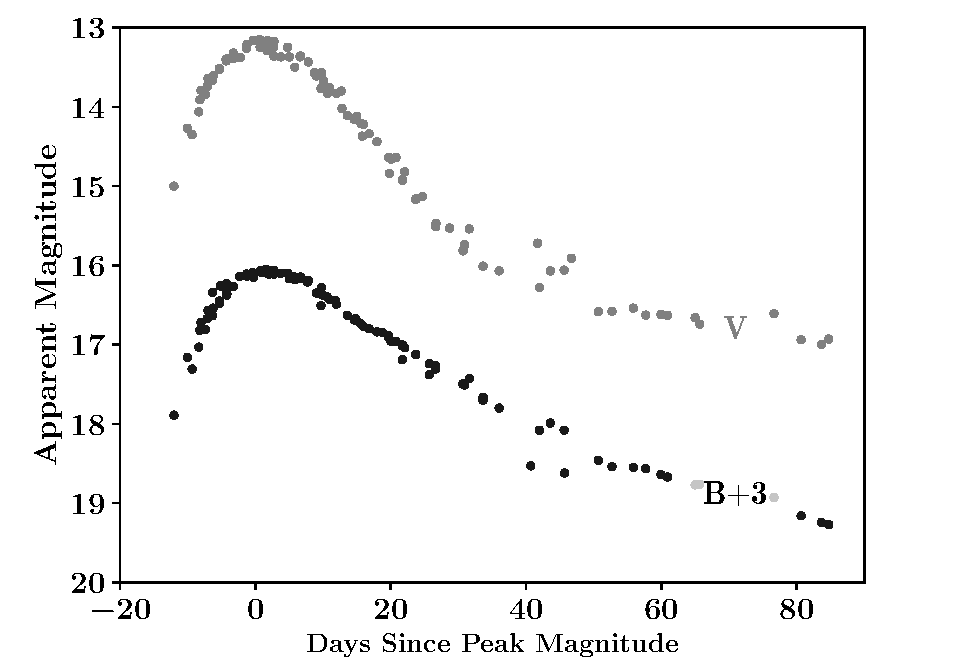
\includegraphics[width=9.25cm]{intro/typeia}
\caption[]{Plot showing the general forms of Type Ia supernovae in the B and V bands. Archival data was translated along the time and magnitude axes to produce the general forms of the light curves. The B band has been offset by a magnitude of $3$ to allow us to see both graphs clearly. The supernovae which were used to plot this graph are: \em{1994ae, 1994S, 1995bd, 1996bo, }\em  and \em{1998aq }\em \cite{jha, matheson}. }
\vspace{-3ex}
\label{fig:typeia}
\end{center}
\end{figure}

In understanding how the consistency of Type Ia light curves arise, we must explore the mechanisms of the explosion. This will involve developing an understanding of the event pre-supernova and also post-explosion.

The general consensus for Type Ia pre-supernova, as discussed by B. W. Carroll and D. A. Ostlie \cite{mod_ast}, is that a white dwarf within a binary system accretes matter from a donor star. However, this is also the initial system for dwarf novae and classical novae, which can be grouped together as cataclysmic variables or novae. These too increase in brightness (classical novae by a factor of $\sim 10^6$ \cite{mod_ast}) which can lead to some confusion with supernovae, especially if you observe them optically without following up with spectroscopic observations. 

It is understood that the difference which leads to Type Ia supernovae and not cataclysmic variable is the process of accretion. This is generally dependent on the binary companion star: if the secondary star is on the main sequence then the white dwarf would just be steadily burning hydrogen or helium in it's surface layers, thus we would just have a cataclysmic variable. To produce a supernova explosion we require a progenitor star which has a mass towards the Chandrasekhar limit ($1.4$ $M_{\odot}$) \cite{posn, longair}. 

If the primary white dwarf was to accrete matter continually from it's binary companion until it itself was brought to the critical mass limit, then a collapse to a neutron star must occur. This is not the case though for a Type Ia supernova, before the white dwarf has a chance to collapse, the star is suddenly disrupted by a large amount of energy.

We can attribute this energy release to the nuclear fusion of carbon and oxygen within the core of the white dwarf. As material is continually accreted and compressed onto it's surface, the star is heated and the temperature increases to $10^9$ K \cite{longair}. When the thermonuclear energy is released, the white dwarf loses it's electron degeneracy pressure, and so becomes gravitationally unstable \cite{longair}. This disruption of the star prevents a total collapse into a neutron star, and instead leads to a supernova explosion \cite{posn}. 

In performing spectroscopic observations of Type Ia supernovae at maximum light we see that intermediate mass elements such as silicon, calcium, magnesium, sulphur, and oxygen are present which supports the picture of thermonuclear disruption \cite{longair, mod_ast}.

The process continues until the heaviest element that nuclear fusion can produce is made, iron. It is created when nickel captures an electron through electron-capture (ec) and turns into cobalt, then the cobalt captures another electron and subsequently $\beta^{+}$ decays into iron \cite{mod_ast}. The process can be summarised in the following equation:
\begin{equation*}
\ce{^{56}Ni} \xrightarrow{\text{ec}} \ce{^{56}Co} \xrightarrow{\text{ec, $\beta^{+}$}} \ce{^{56}Fe}.
\end{equation*}

With these processes, they can be used to explain the form of the Type Ia light curves. The luminosity at peak maximum can be explained as the energy which has been deposited into the expanding envelope from the decay of the \ce{^{56}Ni} nuclei \cite{mod_ast}. 

We can highlight other features of the light curve: the climb to peak magnitude, there is an increase of roughly half a magnitude a day; and with the maximum of the light curve it can be approximated as a Gaussian function \cite{mod_ast}. 

On the other hand, there are some peculiar types of Type Ia supernovae. For example, as featured in Table \ref{table:sn_classes}, Type Ia-91bg are a class of supernovae which have spectra which resembles those of Type Ia, but they have an absorption band at $400-450$ nm. This arising due to a blend of Fe-group elements which are dominated by Ti II \cite{obs_phys_class_sn}. With their light curves they also lack the secondary maximum as found in normal Type Ia's within the I and R bands, features we previously noted as not being in the standard B and V curves.

Observing objects and recognising that they are Type Ia supernovae thus requires not only spectroscopic observations but also observations in the optical. 

\vspace{-3ex}
\subsection{Supernova Discovery}
\vspace{-2ex}
In attempting to discover supernovae it is important that the search is not confined to a single region of the sky, whilst it may be possible to discover one of these events within that region, it would perhaps take a very long time until it would actually occur. What is required is a purpose built supernova survey which spans the entire sky. 

A general method which can be employed to discover new supernovae is one which involves data comparison. If a survey takes an image of the entire night sky for every night, to find new supernovae all that would be required is to subtract one night's data from the previous' and any objects which remain would be objects that could be new supernovae \cite{assasn-rev}. In reality it is not that simple, frames need to be cleaned of noise and they also require to be transformed in response to the spread of the object (the point spread function, PSF). Plus, follow up observations would have to be made to verify if an object is a supernovae or whether it is another transient such as a cataclysmic variable. 

One such survey which employs these methods is the \em{All-Sky Automated Survey for Supernovae }\em (or ASAS-SN). Built up of five observations stations around the world, they are able to view around $48,000$ square degrees of the night sky up to a depth of $\sim 17$ mag \cite{asn_lc}. ASAS-SN is therefore able to find many more supernovae and also supernovae which are close to the cores of galaxies, vastly increasing the discovery rate of bright supernova explosions and improving our understanding of where these events occur.

We note that a large number of their discovered supernovae are close enough to their detection limit that they need to be validated by other astronomers \cite{asn_lc}. This human review of transients has led to projects such as \textit{Supernova Hunters} \cite{cit-sci}, a citizen science program where volunteers are asked to classify objects which could be potential supernova candidates.  

These programs do not detract from the work that astronomers have to perform in the classification of supernovae, but it is important as it allows for the improvement of neural networks which means that automatic surveys such as ASAS-SN could eventually work more autonomously and efficiently \cite{cit-sci}.  

\vspace{-3ex}
\subsection{Application to Cosmology} \label{appcosmo}
\vspace{-2ex}
Once observations for Type Ia supernovae have been obtained, light curves can then be produced. Through the conversion of a time series of photometric observations into a set of model parameters for each supernova \cite{sn_consts}, these results can then be employed in cosmology. 

We find that before corrections have been applied for the correlation between maximum luminosity and the width of the light curve about maximum luminosity \cite{longair, abs_phil}, the dispersion of the absolute magnitudes at peak for Type Ia is less than 0.5 magnitudes. Once the previous correlation had been accounted for, we find that there is little dispersion and the light curves lie on top of one another in a homogeneous nature. 

With this in mind, if a new Type Ia supernova is discovered and enough data had been collected from it to produce a light curve, using that and the width-luminosity relation it would be possible to calculate their absolute magnitudes, thus they can be used to determine the redshift-distance relation \cite{mod_ast}.

For example, if we had a sample of nearby Type Ia supernovae with redshifts of $\mathrel{\mathsmaller{\lesssim}} 0.1$, we could derive a value for Hubble's Constant by plotting them on a Hubble diagram \cite{exp_uni_sn}, and in turn use a rearranged form of Hubble's Law,
\begin{equation}
H_0 = \frac{v}{d}, 
\label{eqn:h_0}
\end{equation}
where $H_0$ is the value for Hubble's Constant, $v$ is the recessional velocity of the supernova, and $d$ is the distance to the supernova \cite{mod_ast}. 

To calculate the recessional velocity, the redshift of the supernova has to be obtained, this could be obtained by making spectroscopic observations, and then $v$ would be calculated with,
 \begin{equation}
v = zc,
\label{eqn:redshift}
\end{equation}

where $v$ is the recessional velocity of the supernova, $z$ is the redshift of it, and $c$ is the speed of light in a vacuum \cite{mod_ast}.

Extending the usages of Type Ia's in cosmology, we see that they could also be used to provide statistical constraints on cosmological models. For example for an $\Omega_M$, $\Omega_{\Lambda}$ Universe, wwhere $\Omega_M$ is the mass density which includes ordinary and dark matter, and $\Omega_{\Lambda}$ is the effective mass density of dark energy \cite{mod_ast, exp_uni_sn}. Additionally, the time-averaged equation of state of dark energy, $w$, could be measured \cite{sn_consts}. This is a value which can then be used to characterise the state of the universe - for an accelerating, dark energy dominated universe we would find that $w \approx -1$ \cite{longair}. 

We thus find that Type Ia supernovae are a very useful tool which can be applied within cosmology.

\vspace{-3ex}
\subsection{Project Aims}
\vspace{-2ex}
This paper discusses the study that was undertaken to observe Type Ia supernovae using ground based telescopes, to learn about the different approaches which can be employed in fitting template light curves onto collected data, and then to evaluate the quality of the results that these methods provide.

In Section \ref{obsver} we describe how we collected and analysed our supernova data, and how we accounted for the uncertainties that arose during the experiment. Our final light curves, and the methods that were used to fit models to the observations is summarised in Section \ref{analysis}. Then in Section \ref{discussion} we further discuss the model fitting, primarily our usage of the fitter program, \textit{SNooPy}, we question and analyse the quality of fit produced and whether we could use our results for supernova cosmology. We end on a discussion of our extension work.

\vspace{-3ex}
\section{Observations} 
\label{obsver}
\vspace{-2ex}
\subsection{Data Collection}
\label{observer-collection}
\vspace{-2ex}
To observe supernova explosions our main pieces of experimental equipment were telescopes which had been fitted with CCD cameras.

We employed three out of the four telescopes based on the Department of Physic's Roof in Durham, and also the robotic telescope on the roof of the William Herschel Telescope building at Roque de los Muchachos Observatory in La Palma.

For the vast majority of our observations we used the 16$''$ telescope (Far-East-16, or FE16) from the Durham array and the robotic 0.5 m telescope (pt5m) from La Palma. We used these two telescopes predominantly as they allowed us the best resolution and illumination on our faint objects. Compared to the 14$''$ telescopes (West-14 and East-14) which are also part of the Durham array, having a larger aperture means that a more sufficient number of photons could be obtained so that we could study our targets more effectively. 

Both Far-East-16 and pt5m use variants of the Cassegrain Telescope, they are Ritchey-Chr\'{e}tein (RC) Telescopes. This derivative is composed of a hyperboloidal primary and secondary mirror \cite{tel_tech} as can be seen in Figure \ref{fig:cass_spec}. With this design, the telescope can produce good quality images over a field of view of several tens of arcminutes across as opposed to just a few minutes of arc when a basic Cassegrain design is used \cite{tel_tech}. 
\begin{figure}[!h]
\begin{center}
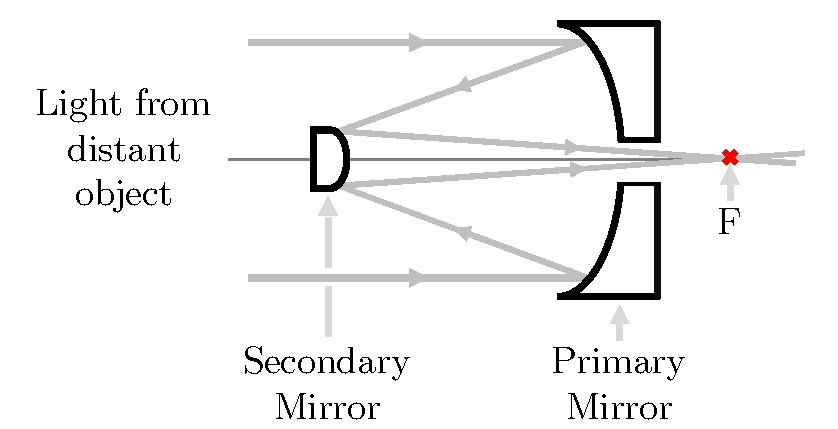
\includegraphics[width=7.5cm]{observations/cassegrain}
\caption[]{A schematic overview of a Cassegrain/Ritchey-Chr\'{e}tein Telescope. In a Cassegrain, the primary mirror is paraboloidal, and in the Ritchey-Chr\'{e}tein the primary mirror is hyperboloidal. In both types the secondary mirror is a convex hyperboloidal. We note F in the diagram is the focal point of the telescope where a CCD camera can be placed. \\ (\textit{This diagram has been adapted from Telescopes and Techniques} \cite{tel_tech}.)}
\vspace{-1.5em}
\label{fig:cass_spec}
\end{center}
\end{figure}

To record and make use of the collected light from our supernova targets we had to use CCD cameras which were mounted at the focal points of our telescopes. On Far-East-16, a QSI 583ws CCD was used with an LX200R telescope, and with pt5m a Kodak KAF-3200ME CCD with an Officina Stellare 0.5m Ritchey-Chr\'{e}tein telescope. In a simplified manner, these CCD cameras would convert the photons into electrons and then the electron signal would be processed by a computer into an image \cite{mod_ast, tel_tech}. This could then be manipulated and analysed using astronomical software packages such as \textit{GAIA} \cite{starlink}.

For our project in particular, we wanted to produce light curves of supernovae within different colour bands. By using photometric filters on our CCDs we were able to observe supernovae within other bands. In doing so, we would be viewing specific wavelengths of light from our objects, this corresponds to particular energies in the different elements present in astronomical bodies \cite{astro_filters}. 

Once we had selected our photometric filters and began our observations, we had to be acutely aware of the possible over-saturation of the CCDs. As our objects were faint and observing conditions could often be bad, we had to collect as much light as possible before our images became oversaturated due to a brighter object within the same field of view. This would be mitigated by lowering the time that we would be observing for, thus there would be less photons collected from the secondary object.

In spite of this, having just one image of our faint supernovae to analyse would not be representative of it's magnitude. Through the process of image stacking (see Section \ref{observer-observations}) we were able to improve the quality of the image by compositing together several images of the same area of sky. Thus it was beneficial when we were observing to take multiple exposures for our objects with the same exposure time and repeating for each photometric filter that we were going to use. 

As we progressed through our experimental period we came to realise that astronomical observations are heavily reliant on weather conditions. What happened to be occurring in the atmosphere that night would have an influence on what you could see with your telescope. This overall effect of the atmosphere on images taken is called \textit{seeing} \cite{tel_tech}.

In the first instance, having a night sky without any visible clouds would be a good initial step. Once the conditions appear to be clear, the atmospheric turbulence would have to be considered next. This is the process when air is turbulently mixed together at different temperatures, thus creating cells or pockets which have different refractive indexes when compared to their surrounding areas \cite{princ_stell_inter}. The effect of this is to produce an image which is blurred and is of lower quality.

In quantifying this seeing as a value, the full width at half maximum (FWHM) can be given for each observation made. The FWHM is a resolution criterion which can be defined as, \textquote{the diameter of the Airy disk at half of its maximum intensity} \cite{princ_stell_inter}. The Airy disk being the central spot of the diffraction pattern which occurs when light from a distant point source has been diffracted by a circular aperture, say, by a telescope. 

Given in arcseconds, the best observing sites produce a stellar image about $0.25''$ across, for an average site it will be typically $2''$ \cite{tel_tech}. What we found was that for Far-East-16, our seeing ranged from $3''$ on a clear night to $\sim6''+$ on a cloudy and turbulent night. For pt5m, we found that seeing was generally better on good nights as it is in a purpose location for astronomical observations: it is away from light pollution and has better atmospheric conditions than in Durham.

To account for atmospheric turbulence and distortions, one could use an adaptive optic system. For example, an artificial laser guide star could be created and projected near to the targets, then the amount that it is being perturbed by can be applied to the main object that is being observed \cite{princ_stell_inter}.

However, as Far-East-16 and pt5m are not equipped to perform these measurements, we could not account for these disturbances. As a result of this, we had to choose nights when the wind was calm, and at times the telescopes had to be refocussed to adapt to the changing atmosphere.

We note that this latter solution was only possible when we were observing in Durham (and not La Palma) as the CCD settings could be manually altered on the fly from the Durham control room.

During our observations bad seeing due to changing weather conditions was not the only factor which would affect us and which we could not account for. Light pollution is a common problem in astronomy and we were no exception to it. With Far-East-16, as the telescope is elevated onto the Department of Physics' roof, light pollution from the majority of the City of Durham could be avoided. Difficulties would arise when our objects were in the night sky above Durham Cathedral. This historic building uses spotlights to illuminate parts of itself, and some of this light inevitably bleeds off into the sky creating a halo of light - something not beneficial for magnitude based observations.

Similarly, if our targets were within $40\degree$ or less to the Moon on the celestial sphere, then observations would not be possible as the reflected sunlight would create a similar disc or halo of light and completely drown out our supernovae. This effect would especially be magnified if the Moon was in a Full Moon phase.

We thus find that there are multiple factors which we have to be aware of and also consider when performing our observations. From the types of photometric filters to weather conditions, there are several components which contribute to the final data set that we collect.

\vspace{-3ex}
\subsection{Observations Made}
\label{observer-observations}
\vspace{-2ex}
Over a period of 34 days we made observations of 19 different objects, some Type Ia supernovae, a few Type II, and some cataclysmic variables. These objects are noted in our objects log in Appendix \ref{app:objects_log}, and our individual observations from the entire experiment are detailed in Appendix \ref{app:observations_log}.

It was realised early on in our project that it would not feasible for us to track multiple objects for an extended period. This was firstly because observation time had to be distributed equally amongst all the projects within the laboratory, it would be unfair to observe just supernovae for an entire night; secondly with such a large amount of data, we would not be able to process or analyse it all; and thirdly, some of the targets were just not worth observing at all. These objects would be too close to their host galaxy, or they would be too low on the horizon for the telescopes in Durham or La Palma to view them.

In choosing which objects to observe we used the \textit{Rochester Bright Supernova} \cite{rochester_sn} and \textit{ASAS-SN Supernovae} \cite{asassn_sn} Lists. These are databases which are updated by astronomers with the latest discovered supernovae. For our observations we aimed to choose supernovae which had a discovery magnitude of around 18 mag or less, anything greater than this would be too faint to observe with our telescopes.

After reviewing our initial data and considering which objects would provide the best basis for producing Type Ia light curves, we chose two supernovae targets: 2017hhz, a Type Ia in galaxy UGC 01218; and 2017hle, a Type Ia-91bg in NGC 0387. Both being not too close to their host galaxy's nucleus and from the lists they appeared to be the brightest supernova objects discovered at the time.

However, they were still quite faint so we had to vary the exposure time between 60s and 120s, and often take more than 4 exposures for each band. In doing so we would later be able to improve the quality and brightness of the supernovae seen in the image through noise reduction and image stacking.

\vspace{-3ex}
\subsection{Data Analysis} \label{data_analysis}
\vspace{-2ex}
As we continually collected data over the experimental period, we had to simultaneously analyse it to ensure that the magnitudes we were obtaining would be useful in supernova light curves.

Photometry was thus performed on each of our frames. Our goals with this were to: take our supernova images, reduce unwanted noise, and then obtain a value for the magnitude with an associated uncertainty. After this, we could use these values in template fittings, and then attempt to perform cosmology.

So, taking our raw frames we firstly had to reduce the noise from unwanted sources. Two sources which we did not have to consider directly was the bias and dark current. The bias arose due to the readout of the CCD, noise is normally created when it is converting the captured photon signal from analogue to digital \cite{obs_uni}. To account for this, bias frames of zero second exposures were taken and subtracted from the data before the data is stored. On the other hand, dark current is the creation of electrons due to the thermal energy of the CCD \cite{obs_uni}. This was remedied by cooling the chips to about $-10\degree$ C, preventing any such noise from forming and being included in the total signal.

The CCD produced one other type of noise which was taken into account. Each pixel on the CCD varied slightly from one another in terms of it's sensitivity, something that arose due to the manufacturing process. This sensitivity was removed by producing and using frames of a uniformly lit area, `flat-fields'. The twilight sky was imaged, and this was then subtracted from our data. The inside of the telescope dome could also be imaged and used for this.
 
Finally, noise such as cosmic rays was removed from our data by stacking (combining) multiple frames of the same field and same exposure time together. This is a process where the median value for each pixel is found from the stack of images, thus any anomalously high values which arise due to cosmic rays can be removed.

Once our frames had been cleaned of noise we then began to perform photometry, more specifically, aperture photometry. After identifying the supernova in our images, we wanted to calculate the apparent magnitude and see how it progressed with time. To perform this we firstly had to choose (at least) two calibration stars, they had to be of similar size to the supernova and be in the general proximity of it.  This was so that when performing aperture photometry a similar `signal' could be obtained across all objects and a similar sky background noise could be obtained as well. Noise which arose from the night sky and which could not be directly removed through subtraction techniques.

Another important criterion for these calibration objects was that their apparent magnitudes had to be known already. This was required for the calculation of the supernova magnitudes. So, we used the \textit{UCAC4 Catalog} to find the photometric data for our calibration stars in the B and V bands. For the 2017hhz frames we chose calibration stars 512-002598 and 512-002599, and for 2017hle we used 613-003374 and 613-003367. These names are the identifiers that are used by UCAC4. Once we had our data and calibration objects, we then used the following equation, 
\begin{equation}
    m = z - 2.5 \log_{10}{C},
\label{eqn:mag_counts}
\end{equation}

where $m$ is the magnitude of an object, $z$ is the zero-point of the frame, and $C$ is the number of counts we receive from said object \cite{astro_image_processing}.

In using this equation we first required the zero-point for the image that we were working with. As what we imaged would not contain the actual magnitudes of the objects, instead they would be offset by a certain amount, $z$, due to factors such as the light being absorbed by dust in the supernova's host galaxy, through the interstellar medium, and by the dust that is in our own galaxy.

We therefore began by measuring the counts $C$ for the calibration stars. With this and their apparent magnitudes $m$ we could solve Equation \ref{eqn:mag_counts} for $z$. Once this was done for each star in each required band, the $z$ values were then all averaged together within their respective observation bands. This zero-point was used with the number of counts for the supernova to produce an apparent magnitude for it.

With obtaining a value for the counts, whether from the supernovae or from the calibration objects, we had to choose a fixed aperture size to count the signal that was contained within it and a fixed sky annulus to count the sky background noise. It was important that the radius of both the aperture and sky annulus would maximise the signal whilst reducing the amount of sky noise measured.

This was done by selecting one of the calibration stars and then plotting how the signal-to-noise ($S/N$) ratio would change as the radius was increased. Derived from High Energy Astrophysics \cite{longair}, we used the following equation for the signal to noise,
\begin{equation}
\frac{S}{N} = \frac{N_{\gamma}}{\sqrt{N_{\gamma}+N_{b}+N_{d}+R^2}},
\end{equation}

where $N_{\gamma}$ is the signal of the star, $N_{b}$ the sky background noise, $N_{d}$ the noise due to dark current, and $R$ the readout noise. The latter two sources of noise were reduced and could be ignored from the calculations.

In Figure \ref{fig:2017_stn}(a) we show the $S/N$ plot that was created for the 2017hhz frames, the calibration star (512-002599) was selected from the V band data from the 20th October 2017 as it had the least noise out of all the data we had taken already.
\begin{figure}[!h]
\begin{center}
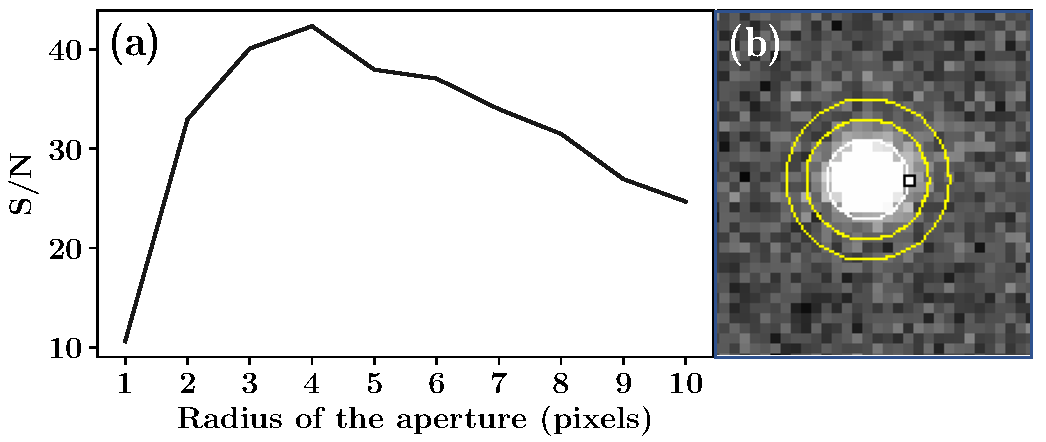
\includegraphics[width=8.5cm]{observations/2017hhz}
\caption[]{(a) Plot of signal to noise against the radius of the aperture for 2017hhz frames, this was used to identify which fixed radius to use. (b) Image of the aperture tool used: inner white circle around star is the main aperture, the outer yellow annuli is used to measure the sky background. Object shown is the star 512-002599.}
\vspace{-5ex}
\label{fig:2017_stn}
\end{center}
\end{figure}

The point where the plot decreases was chosen to be the radius as this would produce an optimal value for the signal to noise. In the case for 2017hhz this was chosen to be 4 pixels and for 2017hle it was 3 pixels. 

Figure \ref{fig:2017_stn}(b) shows the aperture tool that was used extensively for the aperture photometry. With the white circle as the main aperture we counted our object signal from, and the two outer yellow circles being the sky annuli for the sky noise. The area enclosed in the sky would be sampled and then as quantified amount of noise, it would be removed away from the main value for counts. The size of these sky rings were chosen as the radius scaled by factors $\times 1.5$ and $\times 2$. These numbers were justified as we wanted to avoid taking other stars as part of the sky background, and whilst this did mean we had to take part of the galaxy when we were working with our supernovae, we chose to favour our calibration stars as it was difficult to balance having only noise in the sky area.

For the placements of these apertures, we took a histogram profile of the vertical and horizontal directions of the object, and then placed the centre of the aperture to the location of the peak. 

After we had calculated magnitude values we could then proceed to plot supernova light curves with our data, the process of which can be found in Section \ref{supernovae_models}.

\vspace{-3ex}
\subsection{Data Uncertainties}
\vspace{-2ex}
Throughout the experiment it was important that we kept in mind the uncertainties which could affect the accuracy of our results. Various steps were undertaken to ensure that the sources of errors could be reduced, some of these methods have already been detailed in Section \ref{data_analysis}, however we would like to discuss other random and systematic uncertainties.

In collecting data, we have already learnt how a CCD could count extra noise in the forms of bias and dark current if it is not accounted for. Alternatively, we found that as our Type Ia supernovae progressed along their evolutionary path, it became increasingly difficult for us to produce a precise result as they became dimmer and dimmer. This random error is a result of the observational limits of the telescopes, they could only observe to a certain magnitude thus it would be expected that the magnitudes calculated would have a larger uncertainty.

Having access to a larger telescope, one with a greater aperture would allow us to collect more light and thus produce a more accurate and precise value for the supernova magnitudes.

If we consider the systematic errors of our experiment, the greatest source would be as a result of our aperture photometry. Whilst we tried to ensure that we used a set method and set conditions, we may still have accidentally misplaced the positioning of one of the apertures. 

We chose to perform the photometry manually, however to reduce the potential systematic error, we should have automated the process with a script. In doing so, we would be more certain that the counts and magnitudes that we obtained would be more accurate to the true value of the magnitude of the supernova.

On the other hand, we could have repeated the photometry and then took an average value for the counts to reduce any random and systematic errors which may occur. However, as we tried to ensure that our apertures were on the position of peak brightness for our objects, in theory, the results should be the same.

\vspace{-3ex}
\subsection{Final Data}
\vspace{-2ex}
Tables \ref{table:2017hhz_data} and \ref{table:2017hle_data} contain the final calculated magnitudes with their associated uncertainties. Equation \ref{eqn:mag_counts} was used to find the magnitudes, and Equation \ref{eqn:mag_uncert} for the uncertainties - both sets of values use units of magnitude. From this we could then plot Type Ia supernova light curves and attempt to perform cosmology with the results.

\begin{table}[h!]
\centering
\begin{tabular}{c@{\hskip 20pt}c@{\hskip 20pt}c@{\hskip 20pt}c@{\hskip 20pt}c} 
 \hline
 \textbf{Date Observed} & \textbf{$\boldsymbol{m_B}$} & \textbf{$\boldsymbol{\alpha_{m_B}}$} & \textbf{$\boldsymbol{m_V}$} & \textbf{$\boldsymbol{\alpha_{m_V}}$} \\ [0.5ex] 
 20/10/17 & 16.8 & 0.1 & 17.1 & 0.1 \\
 22/10/17 & 16.9 & 0.1 & 16.8 & 0.1 \\
 23/10/17 & 16.8 & 0.2 & 16.9 & 0.1 \\
 26/10/17 & 17.0 & 0.2 & 17.0 & 0.1 \\
 29/10/17 & 17.2 & 0.1 & 17.0 & 0.1 \\
 30/10/17 & 17.3 & 0.1 & 17.1 & 0.1 \\
 05/11/17 & 17.7 & 0.2 & 17.3 & 0.2 \\
 11/11/17 & 18.2 & 0.4 & 17.5 & 0.2 \\
 16/11/17 & 18.6 & 0.2 & 17.8 & 0.1 \\
 17/11/17 & 18.8 & 0.2 & 18.2 & 0.4 \\
 \hline
\end{tabular}
\caption{10 days worth of data was analysed to produce magnitudes and their uncertainties for the B and V photometric bands for Type Ia supernova, 2017hhz. }
\vspace{-0.5em}
\label{table:2017hhz_data}
\end{table}

\begin{table}[h!]
\centering
\begin{tabular}{c@{\hskip 20pt}c@{\hskip 20pt}c@{\hskip 20pt}c@{\hskip 20pt}c} 
 \hline
 \textbf{Date Observed} & \textbf{$\boldsymbol{m_B}$} & \textbf{$\boldsymbol{\alpha_{m_B}}$} & \textbf{$\boldsymbol{m_V}$} & \textbf{$\boldsymbol{\alpha_{m_V}}$} \\ [0.5ex] 
 26/10/17 & 17.8 & 0.3 & 16.8 & 0.1 \\
 29/10/17 & 18.4 & 0.2 & 17.0 & 0.1 \\
 30/10/17 & 18.6 & 0.2 & 17.1 & 0.1 \\
 16/11/17 & 19.5 & 0.3 & 18.9 & 0.2 \\
 17/11/17 & 19.3 & 0.4 & 18.7 & 0.3 \\
 18/11/17 & 19.6 & 0.5 & 18.7 & 0.3 \\
 \hline
\end{tabular}
\caption{6 days worth of data was analysed for the Type Ia-91bg supernova, 2017hle. For the B and V band, their magnitudes are shown with their associated uncertainties.}
\vspace{-1.5em}
\label{table:2017hle_data}
\end{table}

\vspace{-3ex}
\section{Analysis}
\label{analysis}
\vspace{-2ex}
\subsection{Supernovae Models}
\label{supernovae_models}
\vspace{-2ex}
In fitting templates and models to our data, the process could be done manually, however we chose to use the Python package \textit{SNooPy} \cite{car_snoopy}. SNooPy is an automated fitter for Type Ia light curves, it takes magnitude data as an input and then attempts to fit light curves to that data.

For the basic fitting function, \texttt{fit()}, it would only operate if we provided a set of data in at least two different photometric bands out of the passbands of uBVgriYJHK. SNooPY also required the right ascension (RA) and declination (dec) of the supernova in order for it calculate the galactic extinction from Schlegel maps \cite{snoopy_docs}. On top of that, a value for the heliocentric redshift of the supernova was also needed for the fitting, this is because it was required for the computation of the K-corrections in each of the filters provided \cite{car_snoopy}.

The redshift values for our supernovae were obtained from the discovery notes that were attached to their entry's on the Rochester Bright Supernova List. As our objects were Type Ia they generally would be of interest for cosmology, spectroscopic observations would thus often be performed after their initial discovery, and so we could use the redshift that astronomers had obtained. Hence, for 2017hhz we used a redshift of $z=0.0392$, and for 2017hle $z=0.015$ was used.

After SNooPy had managed to apply the template light curves, this fitting could then be exported and plotted. In addition to this, the final parameters that had been selected by SNooPy could be obtained as well. These included the host galaxy extinction (EBVhost), the time for B-maximum in days (Tmax), the distance modulus to the supernova in magnitudes (DM), and the decline-rate parameter (dm15). Values which would become useful in cosmology.

To see the correlations between these four parameters, covariance plots could be produced using the \texttt{fitMCMC()} function with the argument \texttt{plot\_triangle} selected as \texttt{True}. A covariance matrix with the values could be retrieved and then potentially plotted to produce a heat map as an alternative to the triangle plots. 

\textit{A full walkthrough of how SNooPy was used has been provided in Appendix \ref{app:using_snoopy}.}

\vspace{-3ex}
\subsection{Results}
\vspace{-2ex}
After running our data through SNooPy, we were able to produce Type Ia light curves with the \texttt{fit()} function for 2017hhz and 2017hle. In Figure \ref{fig:2017hhz_lc} and Figure \ref{fig:2017hle_lc} we show their respective light curves, their plotted magnitudes and their uncertainties for the B and V bands. Table \ref{table:snpy_summary} provides a summary of the parameters that were used by SNooPy for these \texttt{fit()} fittings.

In Table \ref{table:chi2}, the $\chi^2$ and reduced $\chi^2$ statistics have been calculated for both supernovae, and for both B and V bands. We also provide the average for reduced $\chi^2$ in both bands. 

Figure \ref{fig:covar_plots} shows a fraction of the covariance plots produced by the SNooPy function \texttt{fitMCMC()} for 2017hhz. They display the correlations between the time for B-maximum, the host galaxy extinction, the distance modulus, and the decline-rate parameter. Table \ref{table:snpy_mcmc_summary} additionally shows the parameter output for the fitting made with this function.

With Figure \ref{fig:2017hhz_collage} we provide a collage of two examples of our data, a frame of our analysed data which has been flat-fielded, and our `galaxy subtraction' extension project.

\begin{figure}[!h]
\begin{center}
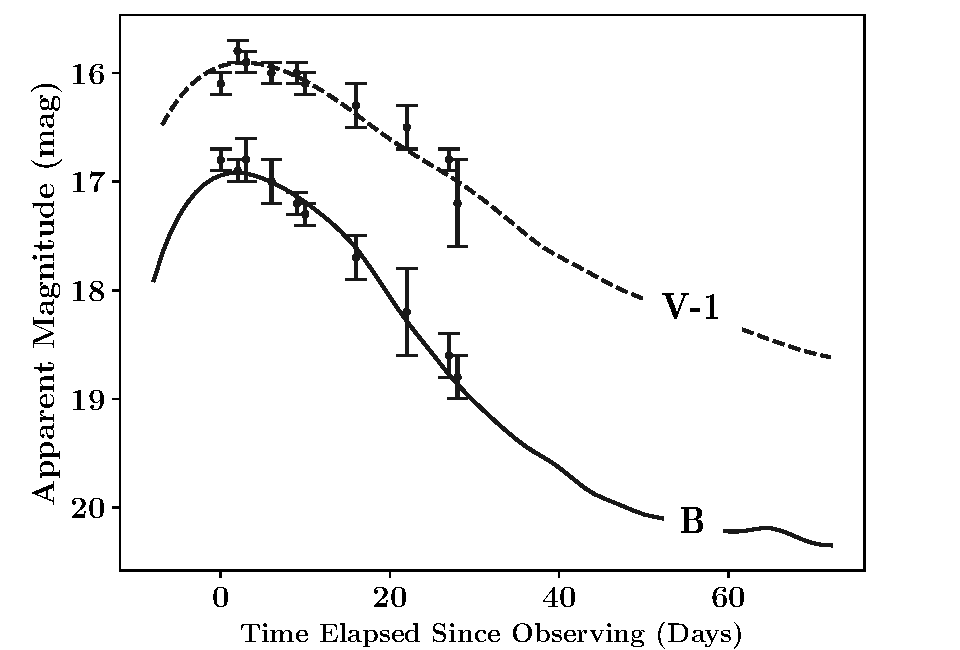
\includegraphics[width=9.25cm]{results/2017hhz}
\caption[]{Plot showing the light curves fitted by SNooPy for supernova 2017hhz. The raw magnitude data has been plotted with their uncertainty in the B and V photometric bands. The V band in this graph has been offset by 1 for ease of viewng. The zero position on the $x$- axis represents the first observation made on Friday 20th October 2017.}
\vspace{-1.5em}
\label{fig:2017hhz_lc}
\end{center}
\end{figure}

\begin{figure}[!h]
\begin{center}
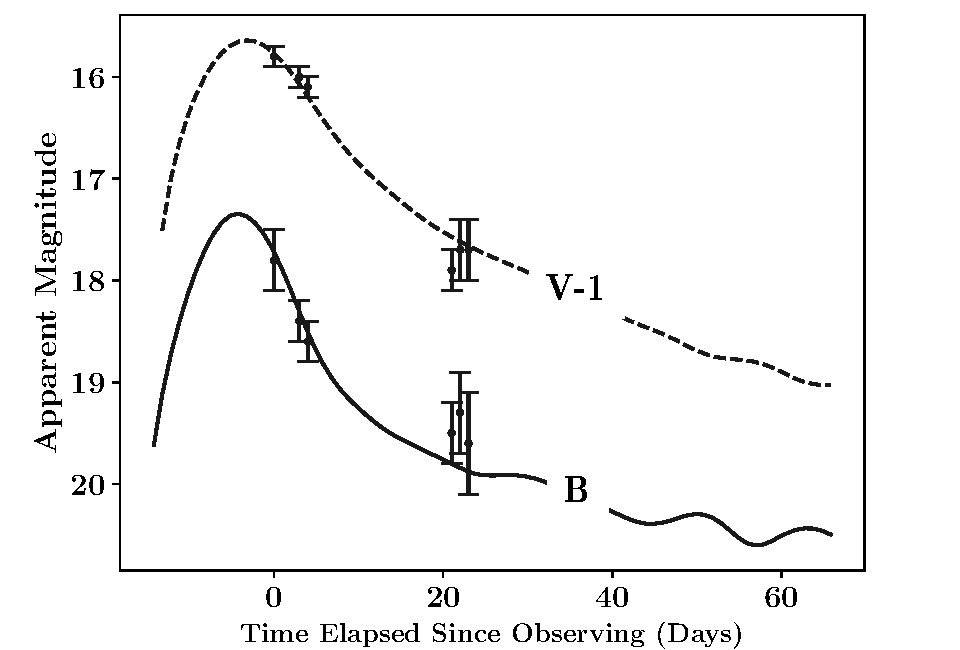
\includegraphics[width=9.25cm]{results/2017hle}
\caption[]{The calculated magnitudes and their uncertainties for the supernova 2017hle have been plotted along with the SNooPy fitted light curves for the B and V bands. The data for the V band in this plot has been offset by 1 to produce a clearer plot. Thursday 26th October 2017 represents the zero point on our $x$- axis.}
\label{fig:2017hle_lc}
\vspace{-1.5em}
\end{center}
\end{figure}

\begin{table}[h!]
\centering
\begin{tabular}{c@{\hskip 15pt}c@{\hskip 15pt}c@{\hskip 15pt}c@{\hskip 15pt}c} 
 \hline
 \textbf{Supernova} & \textbf{EBV} & \textbf{T$_{\boldsymbol{\max}}$} & \textbf{DM} & \textbf{$\boldsymbol{\Delta m_{15}}$} \\ [0.5ex] 
 2017hhz & 0.049 & 2.080 &  36.121 & 0.798 \\
  & $\pm$0.083 & $\pm$1.158 & $\pm$0.106 & $\pm$0.138 \\
  
 2017hle & 0.614 & -3.976 &  34.096 & 1.929 \\
  & $\pm$0.225 & $\pm$1.538 & $\pm$0.455 & $\pm$0.238 \\
 \hline
\end{tabular}
\caption{The parameters that were used by \texttt{fit()} in the fittings of light curves for 2017hhz and 2017hle. Where EBV is the host galaxy extinction in magnitudes, T$_{\max}$ is the time in days for B band maximum since our observations began, DM is the distance modulus in magnitudes, and $\Delta m_{15}$ is the decline rate parameter. These values and their systematic uncertainties have been directly taken from SNooPy's parameter output.}
\vspace{-1.5em}
\label{table:snpy_summary}
\end{table}

\begin{figure}[!h]
\begin{center}
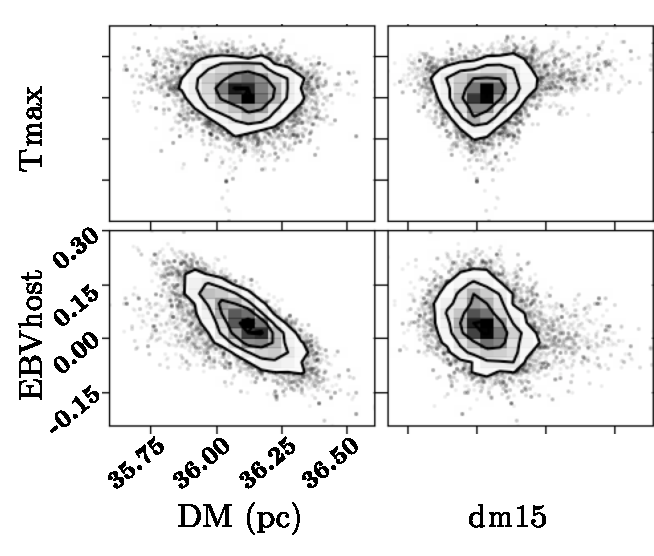
\includegraphics[width=8.25cm]{results/covariance/covariance}
\caption[]{Four out of the six covariance plots produced by the \texttt{fitMCMC()} function for the supernova 2017hhz. The plots show the correlations between four parameters: Tmax, the time for B-maximum; EBVhost, the host galaxy extinction; DM, the distance modulus; and dm15, the decline-rate parameter.}
\label{fig:covar_plots}
\vspace{-1.5em}
\end{center}
\end{figure}

\begin{table}[h!]
\centering
\begin{tabular}{c@{\hskip 20pt}c@{\hskip 20pt}c@{\hskip 20pt}c@{\hskip 20pt}c} 
 \hline
 \textbf{Supernova} & \textbf{$\boldsymbol{\chi^2_B}$} & \textbf{$\boldsymbol{\chi^2_{\nu,B}}$} & \textbf{$\boldsymbol{\chi^2_V}$} & \textbf{$\boldsymbol{\chi^2_{\nu,V}}$} \\ [0.5ex] 
 2017hhz & 5.03 & 0.84 & 8.23 & 1.37 \\
 2017hle & 3.86 & 1.93 & 9.05 & 4.52 \\
 Average & - & 1.38 & - & 2.95 \\
 \hline
\end{tabular}
\caption{$\chi^2$, reduced $\chi^2$ ($\chi^2_{\nu}$) and the average reduced $\chi^2$ values are shown for each photometric filter used in our observations (B,V) for each of our supernovae.}
\label{table:chi2}
\end{table}

\begin{table}[h!]
\centering
\begin{tabular}{c@{\hskip 15pt}c@{\hskip 15pt}c@{\hskip 15pt}c@{\hskip 15pt}c} 
 \hline
 \textbf{Supernova} & \textbf{EBV} & \textbf{T$_{\boldsymbol{\max}}$} & \textbf{DM} & \textbf{$\boldsymbol{\Delta m_{15}}$} \\ [0.5ex] 
 2017hhz & 0.047 & 2.250 &  36.096 & 0.815 \\
  & $\pm$0.067 & $\pm$0.905 & $\pm$0.113 & $\pm$0.076 \\
 \hline
\end{tabular}
\caption{Output of the parameters used for the \texttt{fitMCMC()} fitting. Where EBV is the host galaxy extinction in magnitudes, T$_{\max}$ is the time in days for B band maximum since our observations began, DM is the distance modulus in magnitudes, and $\Delta m_{15}$ is the decline rate parameter. Values and their systematic uncertainties have been quoted in their entirety as used by SNooPy. }
\label{table:snpy_mcmc_summary}
\end{table}

\begin{figure}[!h]
\begin{center}
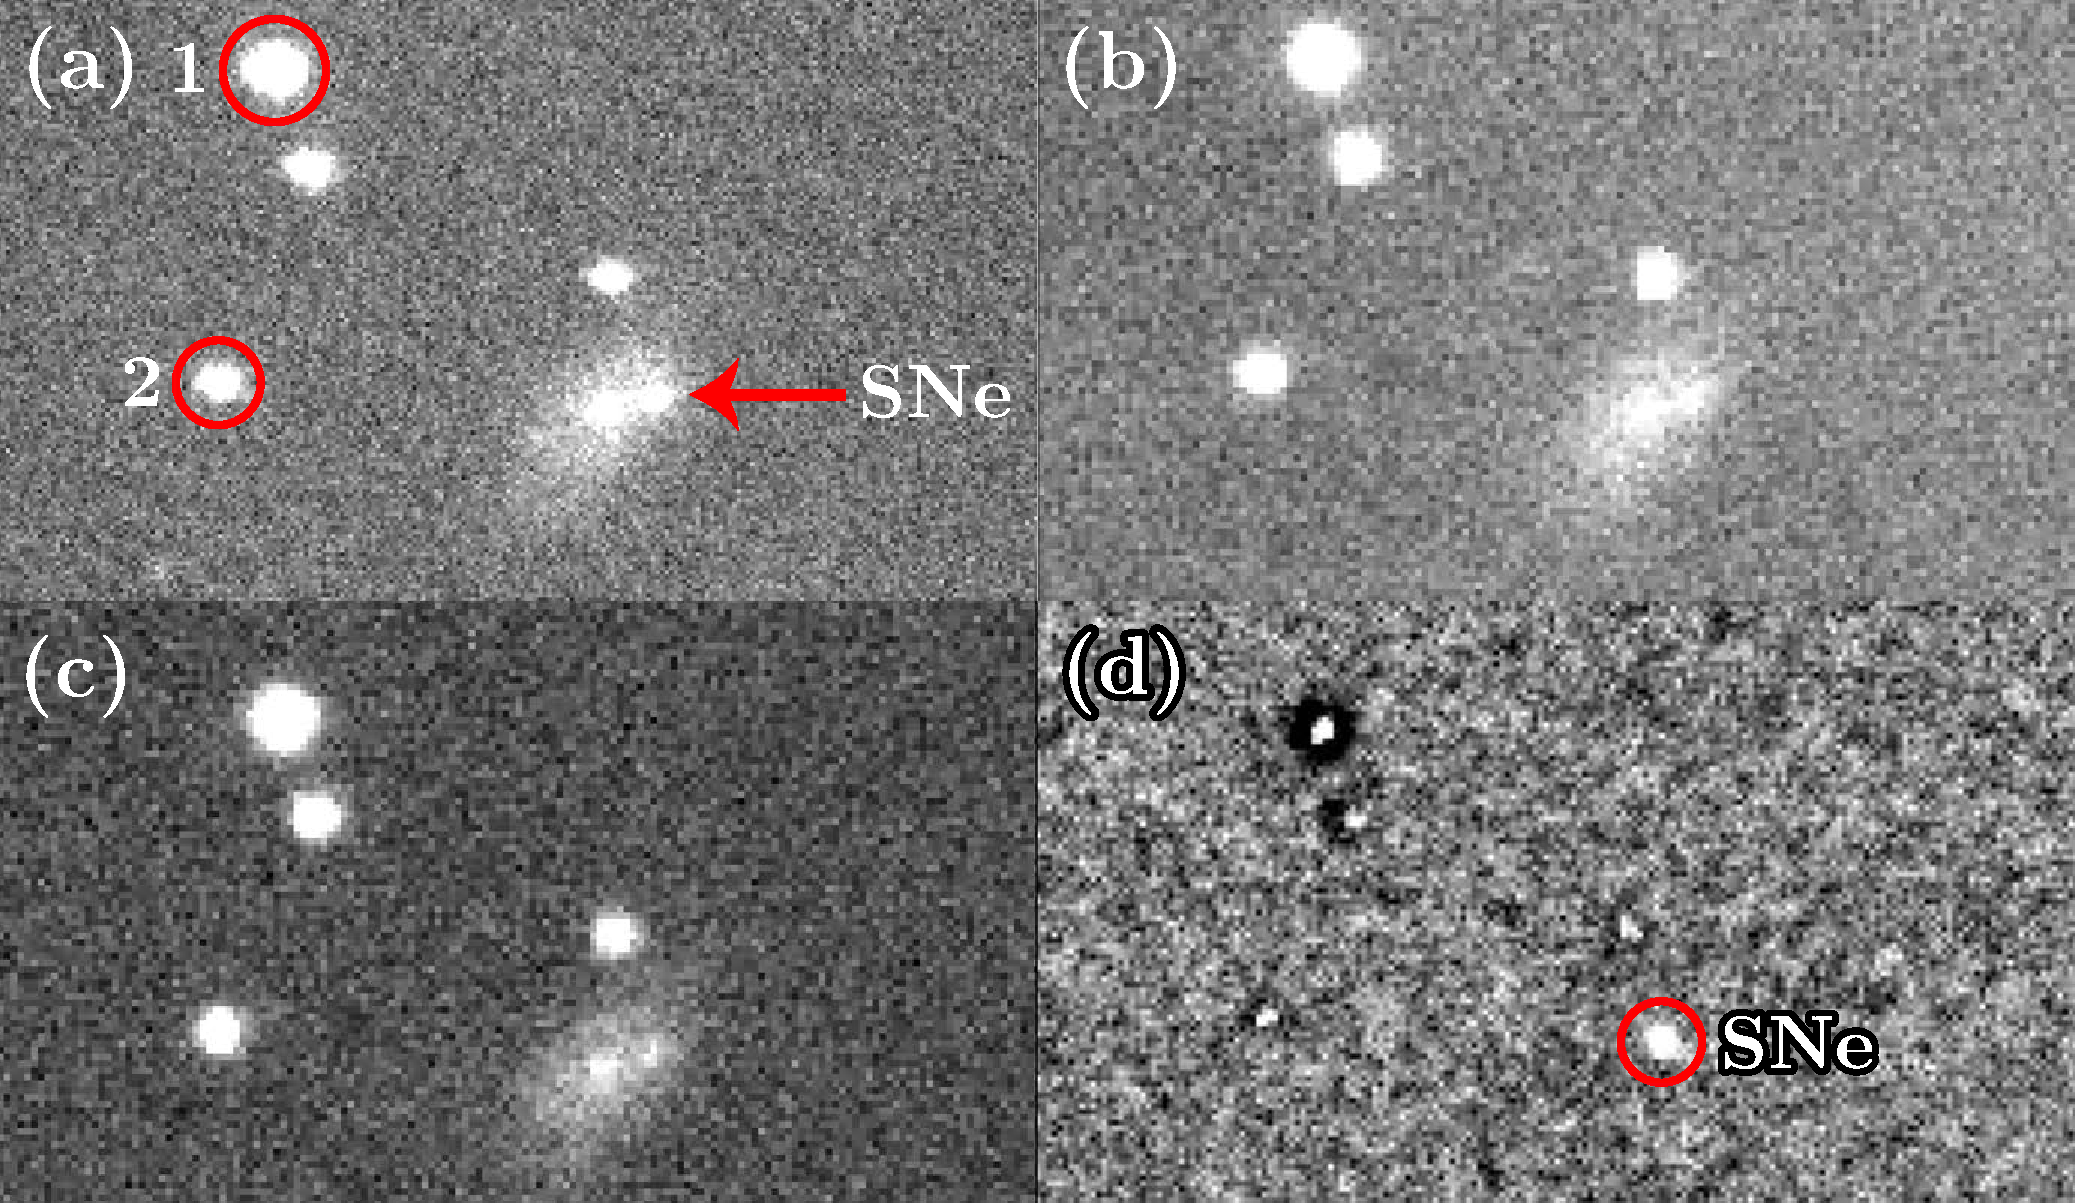
\includegraphics[width=8.25cm]{images/collage_rectangle_small}
\caption[]{V band images of the supernova 2017hhz, it's host galaxy, and the stars in the same field. (a) Our first frame for 2017hhz from the 20th October 2017. The supernova has been labelled as SNe, and our calibration stars, 512-002598 labelled as 1, and 512-002599 labelled as 2. (b) Our last frame of data taken on 23rd November 2017. (c) Data from 23rd November 2017 when flat-fielded. (d) An attempt was made as an extension project to remove the background galaxy for the data from 20th October 2017, supernova 2017hhz has been labelled for your convenience.}
\label{fig:2017hhz_collage}
\vspace{-6ex}
\end{center}
\end{figure}

\vspace{-3ex}
\section{Discussion}
\label{discussion}
\vspace{-2ex}

\subsection{SNooPy, the Type Ia SNe template fitter}
\vspace{-2ex}
\subsubsection{What is the initial quality of the fit?}
\vspace{-2ex}
When we look at the plots that SNooPy produced using \texttt{fit()}, in Figures \ref{fig:2017hhz_lc} and \ref{fig:2017hle_lc} we can initially judge by eye that it appears to be a good fitting, the majority of the points seem to lie on the line within their uncertainties. However if we take a moment, step back, and consider Figure \ref{fig:2017hle_lc}, we see that whilst SNooPy has managed to fit a template to our Type Ia-91bg data, the latter three points in the B band do not appear to have been well fitted at all.

This then raises the following questions, how does this program actually fit templates to data, and how well does it do so? Could we possibly believe and use their final results in some cosmological analysis?

Before we consider the inner workings of SNooPy, we must look at the possibility that the data we collected for those three days was just poor, and this appears to be a likely scenario. With these latter three points, the data was collected around two weeks after our initial observations. The supernova would have more than likely dimmed past the limit to which our telescopes could see. Therefore what we had collected would not have been an accurate representation of the magnitude, and this does show with the template fitting.

Returning to our initial discussion on SNooPy's ability to fit templates, as an initial way for us to compare and contrast different results, we will use the value for the peak intrinsic magnitude in the B band ($m_B$), and the time for this maximum ($t_{\max}$). With this we will introduce Philips' parameter, $\Delta m_{15}(B)$, the mean rate of decline of the B band light curve between maximum light and a time interval of 15 days after peak \cite{abs_phil}. Using this value which we can obtain from SNooPy we can then use the following equation to calculate the peak B band magnitude,
\begin{equation}
M_{\max}(B) = -21.726 + 2.698 \Delta m_{15}(B),
\label{intrinsic_b}
\end{equation}

where $\Delta m_{15}(B)$ is the decline rate parameter \cite{high_en_astro}.

Hence, using Equation \ref{intrinsic_b} and the values from Table \ref{table:snpy_summary}, for our final fittings we find an absolute maximum magnitude of $-19.6\pm0.3$ mag for 2017hhz, and $-16.5\pm0.6$ mag for 2017hle. As a comparison we have calculated this with the \texttt{fitMCMC()} data from Table \ref{table:snpy_mcmc_summary}, $-19.5\pm0.2$ mag. The typical absolute B band magnitudes for Type Ia supernovae is $M_B = -19.5 \pm 0.1$ mag \cite{longair}, which both our 2017hhz values agrees with. Plus for our Type Ia-91bg, Phillips (1993) \cite{abs_phil} finds a value of $M_B = -16.38\pm0.2$ mag which is also in agreement. 

From this, we find that with our data and with SNooPy's \texttt{fit()} fitting we produce absolute magnitude values which lie within the typical values. However, there is still a need to further question the quality of the fit. Earlier in the project, when we did not have the latter three values for 2017hle, we ran the SNooPy routine and found a value $\Delta m_{15}=0.073\pm0.039$ which produces $M_B = -21.5\pm0.1$ mag. Comparing this to our full data set value and Philips' value we see that it is not an accurate value whatsoever. 

We can thus draw our first conclusion about SNooPy (and about supernova template fitting in general), a complete set of data is required to effectively produce a light curve. Data which covers the majority of the evolution of the Type Ia supernova - from before peak magnitude to afterwards when it is in decline. 

Removing the latter three points for 2017hhz and running SNooPy we find, $\Delta m_{15}=1.036\pm0.243$ and thus $M_B = -18.9\pm0.7$ mag. This is more inline with what is typical, we could say this is because we still have seven points which form the general profile of the light curve, a fitting would therefore be more likely to be accurate.

Yet we still have to remain skeptical with our final plots. The positioning of the peak magnitude in the B and V bands is the main contending issue, whilst it appears for 2017hhz we capture our first data when it is at it's peak magnitude, we cannot truly be sure if this is the case. We require more data before that first point on the 20th October 2017. 

We did attempt to add additional points by looking at the initial observations performed by other astronomers. However they were not included as their measurements were made in different photometric bands and we were unsure on how to convert between different systems. 

If we return to our discussion on the quality of the fit, numerically, we can quantify this with $\chi^2$ statistics. It has been defined that a model is a good fit to the data if $\chi^2_{\nu} \approx 1$ (the reduced $\chi^2$) \cite{hugheshase}. From Table \ref{table:chi2} we see that for the B photometric band, both 2017hhz and 2017hle have better fits than their counterparts in the V. Whilst this is a test of the fit of the \textit{model} to the data, we once again cannot detract from the possibility that the data we collected and analysed was inaccurate. Again, potentially due to observation limits, or the frames not being entirely clean of noise, or due to more data being required. The values subsequently produced would naturally stray from unity. 

Since we began this section we have looked at the results which SNooPy created and have drawn basic conclusions on the quality of fit. We have calculated and analysed the absolute magnitudes of the supernovae and also the $\chi^2_{\nu}$ values for the fitting. But, we have not yet explored the implications of the results from \texttt{fitMCMC()}, instead, we would like to first understand the underlying methodology that has been employed by the program, and by extension we could then apply this in our own supernova light curve fitting routine. 

\vspace{-3ex}
\subsubsection{How is the fitting actually performed?}
\vspace{-2ex}

In fitting templates there are many well-established methods which can be employed to fit data in a broad number of photometric bands. We must start though at the beginning, and understand the very basics behind the production and fitting Type Ia light curves.

Within the B and to an extent V-band, light curves can generally be fitted by using a single template which has been stretched along the time axis to fit the observed data \cite{highred_perl}. However, applying this to longer wavelengths becomes more difficult as other features arise. For example, an inflection observed in the r band after 20 days will evolve into a secondary maximum when viewed in the i band \cite{car_snoopy}. More templates have to be derived and produced for the observations made in other photometric filters.

As a result, a single-parameter family of curves became the accepted base method instead of using the stretch-like correction. This single parameter would be used to describe the shape of the light curve and would be employed when the template is being fitted.

One package which we have not used, SALT2 \cite{salt2}, uses a stretch-like parameter $x_1$ to describe a sequence of spectral energy distributions of Type Ia supernovae which is further modified by a colour-like parameter $c$. Another fitter, MLCS2k2, uses a luminosity parameter $\Delta$ to describe their light curves \cite{prec_indic, mlcs2k2}. 

With SNooPy, none of these parameters are used, instead, the decline-rate parameter $\Delta m_{15}(B)$ is employed in the making and fitting of SNooPy's templates. Compared to the other two packages, the advantage that is given for this is that it is a characteristic of the observed light curve which can be easily measured \cite{car_snoopy}. But as it is tied to a particular filter and photometric system, it cannot be truly universal.

Detailed by Burns et al (2011) \cite{car_snoopy}, the initial theory and methods which build on the ideas of $\Delta m_{15}$ are beyond the scope of our understanding and beyond the purpose of this experiment, they cover topics such as: spline fittings, the interpolation of a sample four-dimensional surface, and the fitting of bi-variate polynomial functions. 

What is actually useful for us is that after the creators of SNooPy had created some basic light curve templates, they arrived at the following conclusion:

\textquote{If we use the above procedure to generate a B light-curve template with a particular $\Delta m_{15}$, there is no guarantee that the \textit{measured} change in magnitude of the template from peak to day 15 will exactly match the input $\Delta m_{15}(B)$.} \cite{car_snoopy}.

In other words, for the values of the decline-rate parameter obtained after the fitting had been performed, they would not correspond to the values which were initially used in the making of the templates. If we had then used these templates uncorrected, inaccuracies would certainly arise when calculating $M_{\max}(B)$ for example. 

Building upon this, we noted earlier that it was difficult to accept a light curve which had been fitted for just a few data points. It was recognised by the creators of SNooPy that with a single parameter family of curves, reproducing observations with templates away from maximum light is currently inadequate \cite{car_snoopy}. They suggest that at least another parameter should be introduced in the future to improve the fittings.  

In the mean time, they have just included the intrinsic variations as an extra uncertainty in the template. Additionally, as the fitting of their templates incorporate contributions from every photometric band provided, there is another extra random and systematic uncertainty.

Whilst the decline rate parameter is the main parameter used in the production of SNooPy light curves, fitting them requires the \texttt{fit()} and \texttt{fitMCMC()} functions to find the best fit parameters for not just $\Delta m_{15}$, but for the host galaxy extinction, time for B-maximum, and the distance modulus as well. These four values have uncertainties which incorporate a statistical component as a result of the fittings \cite{car_snoopy}.  

\texttt{fit()} uses a non-linear least-squares algorithm in it's fitting, the Levenberg-Marquardt method. It minimises the variance-weighted residuals of the data from the model \cite{snoopy_online_docs} (it attempts to find the minimum $\chi^2$). 

\texttt{fitMCMC()} on the other hand uses a Markov Chain Monte Carlo (MCMC) approach which provides the advantage of a less biased estimator of the regression parameters, and it can use more sophisticated models of the statistical processes that produced the data \cite{car_snoopy}. 

Considering what we have discussed, we thus find that the main tool used by SNooPy in the fitting of supernova templates is statistical analysis based on optimising various parameters. If we had performed these fittings manually, we most likely would taken the route of stretching of an averaged Type Ia light curve onto our data and then calculate the $\chi^2$ values to see if it would be a good fit or not.

We now arrive at the point where we have some understanding of how SNooPy and template fitters work, we shall therefore return to our earlier discussion on the quality of SNooPy's fitting. 

\vspace{-3ex}
\subsubsection{So, how do we view the quality of the fit now?}
\vspace{-2ex}

As we chose to use \texttt{fit()} as our main tool, we did sacrifice some potential accuracy by not using the MCMC based function. When comparing Table \ref{table:snpy_summary} and \ref{table:snpy_mcmc_summary}, we see that the parameters differ from each other by about $\sim0.06\%$ to $\sim8\%$. Whilst this is not orders of magnitude different, if we had choose between them so that we could calculate some cosmological parameters, we would certainly use the output from \texttt{fitMCMC()}.

Viewing the covariance plots for our fittings, from Figure \ref{fig:covar_plots} we can see that the host galaxy extinction (EBVhost) is strongly negatively correlated with the distance modulus (DM) which does not come as a surprise. As the host extinction (the reddening of the light) increases then the apparent magnitude of the supernova that can be observed decreases. 

With the other parameters, we can see from the covariance plots that they have very little correlation to each other. This can be extended for the relations between dm15-DM and EBVhost-Tmax which we have not presented, they too show no correlations.

The point to make here then is that as they are correlated we should have constrained one of the host extinction or the distance modulus. Instead, we gave SNooPY free reign in finding and optimising the parameters, using methods such as minimising $\chi^2$ and calling up the Schlegel maps to find the extinction with our given RA and dec. 

This does mean that we can now compare SNooPy's output with known information and use this as an extra judge of the quality of fit. Focussing on the results for 2017hhz, we begin with the distance modulus. For \texttt{fit()} and \texttt{fitMCMC()} we get $36.121\pm0.106$ mag and $36.096\pm0.113$ mag respectively, and retrieved from NED the Tully-Fisher determined value for UGC 01218 is $35.64\pm0.43$ mag \cite{tully_fish_catalogue}. Comparing these values we see that whilst they are not completely different, within the SNooPy uncertainties, they do not agree with the Tully-Fisher distance modulus. Noting that the SNooPy uncertainties for host extinction and distance modulus do incorporate systematic errors, for example, the distance modulus includes the intrinsic dispersion of the Phillips relation.  \cite{snoopy_online_docs}.

A similar comparison can be attempted then for the host extinction. SNooPy produced $0.049\pm0.083$ mag and $0.047\pm0.067$ mag, whilst a galactic extinction of 0.043 mag can be quoted from Schlafly and Finkbeiner (2011) \cite{reddening}. As the statistical uncertainties for our values are larger than their companion extinction, this further highlights the need that an initial constraint should have been applied to the templates.

We find that overall, whilst SNooPy is able to produce templates and fit them to a certain degree of accuracy, steps have to be taken to ensure that this accuracy can be further improved. Steps such as providing our own constraining parameters, and also using the MCMC based fitter as that provides a more accurate result than \texttt{fit()}.

\vspace{-4ex}
\subsubsection{Can we use our results for cosmology then?}
\vspace{-2ex}

We therefore have the parameters from our final SNooPy fittings and we concluded that they are not entirely inaccurate, what if we now used them to calculate some cosmological parameters?

Take finding a value for Hubble's Constant, using the data for 2017hhz, we have all the required information: the redshift from other astronomers and our distance modulus from SNooPy. If we took Equation \ref{eqn:h_0}, Equation \ref{eqn:redshift}, and the following equation, 
\begin{equation}
\mu = 5 \log_{10}(d) - 5,
\end{equation}

where $\mu$ is the distance modulus in magnitudes and $d$ is the distance in parsecs \cite{mod_ast}. With this and a value for speed of light in a vacuum from NIST \cite{speed_of_light} we would be able to produce $H_0=70\pm20$ km s$^{-1}$ Mpc$^{-1}$.

Comparing this to existing measurements, $H_0 = 73.24 \pm 1.74$ km s$^{-1}$ Mpc$^{-1}$ \cite{hubble_constant}, we see that whilst it appears to be consistent, the uncertainty entirely negates this fact. In our calculations we have had to estimate the uncertainty on the redshift and use SNooPy's provided statistical uncertainty for the distance modulus.

If we wanted to use our results for cosmology we would firstly have to improve the original accuracy of our fitting and find a value for the redshift which has a known uncertainty.  
 
However, we must be aware that calculating $H_0$ is a partly cyclic process when using results from SNooPy. For the production of the Type Ia templates, cosmological parameters ($H_0$, $\Omega_M$, \& $\Omega_{\Lambda}$) were employed in the calibration of the absolute magnitudes of the Type Ia supernovae sample \cite{car_snoopy}. Whilst these parameters are not used in the actual fitting, we note that they might introduce an uncorrectable bias in our results. 

In answering our question, yes, we could use our results for cosmology, but we would have to introduce improvements and additional uncertainties. 

We now arrive at a point where we have discussed the limitations and have judged the quality of fit that SNooPy provides, and now we turn to our methodologies that were used in collecting and analysing data.

\vspace{-3ex}
\subsection{Observing supernovae}
\vspace{-2ex}

In collecting data for this experiment we had to account for the uncertainties for the bias and dark current, we flat-fielded our data to remove the variations in sensitivity of the CCD pixels, and we stacked our data to improve the supernova signal. 

But from our SNooPy results we see that more would be required to improve our data set. One suggestion that we would like to repeat, is that if we were to repeat this experiment for new Type Ia supernovae, we should attempt to use telescopes with a larger aperture. This is so that we could collect more data as the supernova dims, filling out the decline path and improving the overall accuracy of our results.

On the other hand, an attempt could be make to take even more frames when the supernova dims, and when the time came to combine the data, the fainter signals would be improved.

Using a longer exposure time could also be considered, but then there is a possibility that the images would become saturated and in a situation where our targets are already faint, this would not be ideal.

To account avoid this, it would be helpful to know what the magnitude limit for our telescopes are. A quantifiable value is difficult to produce as observations and data are dependent on the conditions at the time of viewing, exposure time, and exposure number. So to put a certain value is difficult, nevertheless we can use our data and final graphs from SNooPy to try and put a rough estimate on the lowest magnitude which can be viewed.

From Table \ref{table:2017hhz_data}, Table \ref{table:2017hle_data} and Figure \ref{fig:2017hle_lc} we can suggest: as the magnitude reaches around and below $18$ mag the uncertainties increase. While we definitely can attribute this to less photons being detected as the supernova dims, we can additionally suggest that this could be the case due to the telescopes reaching their observation limit. Thus we can give a value of $\sim 18$ mag for the limits of Far-East-16 and pt5m.

In highlighting the differences between the types of data that we collected, in Figure \ref{fig:2017hhz_collage} we present a collage of data that we used. At a first glance of Figure \ref{fig:2017hhz_collage}(c)  we note that flat-fielding our data vastly improves the quality of it. It cannot be seen directly but the vignette effect has been removed, cosmic rays taken out, and the data has reduced noise in general. 

With the comparison of the raw data, the first thing to note is that different observation conditions would have been present when the data was being taken. In Figure \ref{fig:2017hhz_collage}(a) five exposures each taken for 120s had been taken in La Palma. For Figure \ref{fig:2017hhz_collage}(b) the Durham site was used for 24 exposures at 60s each. On both days the conditions appeared to be clear. 

We do notice in Figure \ref{fig:2017hhz_collage}(a) that all the objects appear to be slightly warped like a rugby ball, this potentially could be due to atmospheric turbulence. It was not atypical that our data would sometimes have aberrations such as this. We can cite some cases where potentially a satellite or an aeroplane had transited through some of our frames and it was not until we had stacked multiple frames together that we would notice such a thing had occurred.

This is another advantage for collecting as many frames of our objects as possible. In addition to reducing unwanted noise, we could circumnavigate the problems that erroneous images can bring. 

Looking away from data collection, we can instead suggest improvements which could be made instead to our photometry methodology. We have previously discussed that we performed the photometry manually and this should have been made an automated process. We restate this and further suggest that for our calibration objects we should have used more than two so that the accuracy of our zero-points would be improved, and in turn, our apparent magnitudes.

Now, considering the tools we used for this photometry, GAIA was our main astronomical data analysis package. For the counts of our objects we did not make use of the quoted uncertainty from the program, instead we chose a functional approach which can be found in Appendix \ref{app:uncertainties}. A method opted for as we had control and an understanding of how it worked.

For the sky background values, GAIA was utilised again. Values which we only used for our signal-to-noise calculations when we chose the radius of our apertures. The way in which they were calculated could be changed within GAIA's photometry settings. Our calculations in particular made use of the `clipped mean', a mean which disregards the extreme high and low values. Compared with the standard `mean', there is only a $\sim 0.06 \%$ difference between both values, a difference too small to make a difference in our calculations.

Once we had gained a strong set of skills in analysing data we attempted to apply what we had learnt to other projects. 

\vspace{-3ex}
\subsection{Galaxy subtraction, the search for transients, and closing thoughts}
\vspace{-2ex}

Using the data which we had previously collected, we attempted to perform a `galaxy subtraction' on our 2017hhz frames. Our intention was to remove the background galaxy, UGC 01218, and only leave the bright supernova behind. The method consisted of interpolating two frames, one where the supernova is really bright and one where it has faded from view, then one of the images had to be accounted for the point spread function (PSF) of the other. This involved convolving a Gaussian function with the other frame so that the objects in both had the same `spread'. The images could then be scaled and subtracted from each other. In Figure \ref{fig:2017hhz_collage}(d) we see that our attempt was partially successful. We successfully removed the galaxy, but we did not manage to convolve our Gaussian function by the correct amount, thus leaving behind `negative' objects in the place of the stars. 

If we had been successful in implementing this galaxy subtraction, we then would have rudimentarily attempted our own transients survey. Throughout the project, in addition to our supernova observations, we viewed areas where we thought supernovae may occur. We initially started with stellar clusters, Messier 7 and Messier 10, but we soon realised that there would be a low chance for their stars to go supernova. Instead, we took our observations to a galactic cluster, the Perseus Cluster (Abell 426). 

We had intended to carry out a `background subtract' on our frames, and like the supernovae in galaxy subtraction, new events in this survey would be easily detected. We state our past intentions instead of presenting results as there was just not enough time, it was limited and in the end we decided it would be more important for us to focus our efforts on the main project, producing Type Ia light curves. 

Looking at our objects log and observing logs we find that we observed many more objects than just 2017hhz and 2017hle. However, not everything that we collected could be analysed as it would just take an excessive amount of time to do so. 

We therefore suggest that if this project were to be revisited in the future, it would help if the photometry and the template fittings were automated. In doing so, more time could be devoted to the astrophysics behind supernovae and their applications in cosmology. We also suggest that other fitters should be used as well as SNooPy, namely SALT2 and MLCS2k2, it would certainly be interesting to compare and contrast the uncertainties in their results and also the parameters used when fitting light curves.

\vspace{-4ex}
\section{Conclusions}
\label{conclusions}
\vspace{-2ex}

We asked ourselves at the beginning of this experiment whether it would be possible for us to observe Type Ia supernovae and reproduce their evolutionary light curves. Our conclusion is that it is possible, but the accuracy and uncertainties could certainly be improved. 

Through the usage of SNooPy we managed to apply models to our data which were not entirely unacceptable, producing average reduced $\chi^2$ values of $\sim 1.38$ for the B band and $\sim 2.95$ for the V band. The calculated parameters used in these fittings, namely the distance modulus and galactic extinction, are consistent with known values, however, their uncertainties negate any agreement as the results become meaningless. 

Therefore adjustments must be made to produce more reasonable uncertainties. With our observational method, an extensive data set which covers the entire evolution of the supernova should be collected with a larger telescope. Furthermore, for our analysis, if SNooPy is to be used again for light curve fitting, known constraints should be placed on the templates as this would in turn produce more accurate results.

We conclude on this, Type Ia supernovae are an important tool for cosmology and it is thus important to produce accurate light curves. Armed with a better set of results, one could then achieve more consistent values for the geometry of the universe.

\vspace{-4ex}
\section*{Acknowledgements}
\vspace{-2ex}
We thank Dr. J. Lucey, Dr. M. Swinbank, and U. Dudzeviciute for their continual support which was provided over our entire experimental period. We also thank the staff at the Department of Physics at Durham University for the upkeep of the department's telescope array, and we thank Dr. R. Wilson for the usage of the robotic telescope at La Palma. Finally, I thank Duncan Middlemiss for his patience and partnership during this project.

This research has made use of the CfA Supernova Archive, which is funded in part by the National Science Foundation through grant AST 0907903.

The Starlink software (Currie et al 2014) is currently supported by the East Asian Observatory.

\vspace{-3ex}
\bibliographystyle{abbrv}
\bibliography{supernovae}

\clearpage

\appendix

\twocolumngrid
\vspace{-3ex}
\section{Uncertainties} \label{app:uncertainties}
\vspace{-2ex}
\subsection{Magnitudes}
\vspace{-2ex}
Our magnitude values each had an associated uncertainty which was found by using the following equation,
\begin{equation}
\alpha_{m} = 2.5 \log_{10} \Big(1 + \frac{1}{\sqrt{C}} \Big),
\label{eqn:mag_uncert}
\end{equation}

where $\alpha_{m}$ is the uncertainty on the magnitude, and $C$ is the value obtained for the counts of the supernova explosion. This equation was obtained from \textit{Observing the Universe} [A. J. Norton. \textit{Observing the Universe}, The Open University, 2004].

\vspace{-2ex}
\subsection{$\boldsymbol{\chi^2}$}
\vspace{-2ex}
In comparing the fit of the model to our data we used $\chi^2$ statistics in doing so, we now provide the method which was derived. The equations have been adapted from \textit{Measurements and their Uncertainties} [I. G. Hughes and T. P. A. Hase. \textit{Measurements and their Uncertainties}, Oxford University Press, 2010].

An individual value for $\chi^2$ had to be calculated for each data point and their corresponding value from the model, together these were then summed together to produce a total $\chi^2$ value for each photometric band. The following equation summaries this,
\begin{equation}
\chi^2 = \sum_i \frac{(m_i - m(t_i))^2}{\alpha_i^2}, 
\label{eqn:chisquared}
\end{equation}

where $m(t_i)$ represents the model magnitude from SNooPy's fitting, $m_i$ is the magnitude that we calculated from our collected data and $\alpha_i$ is the uncertainty on that magnitude.

Then to use this as a quality of fit we had to reduce the final $\chi^2$ value using the number of degrees of freedom,
\begin{equation}
\nu = N - \mathcal{N},
\end{equation}

where $N$ is the number of independent data points with $\mathcal{N}$ parameters, this latter value was taken to be the number of parameters that SNooPy used in their fittings.

Finally, the reduced $\chi^2$ values would be calculated as follows,
\begin{equation}
\chi^2_{\nu} = \frac{\chi^2}{\nu},
\end{equation}

where $\chi^2$ is as calculated in Equation \ref{eqn:chisquared}, and $\nu$ is the number of degrees of freedom.

\vspace{-2ex}
\subsection{Hubble's Constant, $\boldsymbol{H_0}$}
\vspace{-2ex}
The following calculations makes use of equations and theories derived from \textit{Measurements and their Uncertainties} [I. G. Hughes and T. P. A. Hase. \textit{Measurements and their Uncertainties}, Oxford University Press, 2010].
 
For our calculation of Hubble's Constant we derived the uncertainty as follows.  

To use Hubble's Law and the redshift-velocity relationship as defined by Equations \ref{eqn:h_0} and \ref{eqn:redshift}, we firstly had to retrieve values for the quoted redshifts for our supernovae. Their entries on the Transient Name Server (TNS) had no associated errors, so we looked at the spectrograph's manual in attempt to find a value. 

We only used one of our objects to calculate $H_0$, 2017hhz, and the `SED Machine' was the spectrgraph which identified it's redshift. According to C. C. Ngeow et al [C. C. Ngeow et al. \textit{The SED Machine: A Spectrograph to Efficiently Classify Transient Events Discovered by PTF}. International Astronomical Union, 290, 2012.] this machine provides a spectrophotometric calibration of $\sim 5\%$. Therefore we took $5\%$ of our redshift value as it's uncertainty. 

Our next uncertainty of concern was the value for the distance to the supernova, not the distance modulus. We derived the following equation for the uncertainty in the distance,
\begin{equation}
\alpha_{d} = 10^{\delta} \times \ln{10} \times \alpha_{\mu}, 
\end{equation}

where $\alpha_{d}$ is given in parsecs, $\delta= ([\mu/1]+1)$ and $\alpha_{\mu}$ as the uncertainty on the distance modulus, $\mu$, as found by SNooPy. 

Putting all of this together, we then find a value for the uncertainty of Hubble's Constant,
\begin{equation}
\alpha_{H_0} = H_0 \sqrt{\Big(\frac{\alpha_z}{z}\Big)^2 + \Big(\frac{\alpha_d}{d}\Big)^2},
\end{equation}

where $H_0$ is the calculated value for Hubble's Constant, $\alpha_z$ is the uncertainty on redshift $z$, and $\alpha_d$ is the uncertainty on distance $d$.

\clearpage

\onecolumngrid
\vspace{-3ex}
\section{Programs created}
\vspace{-2ex}
Accessible from \url{https://community.dur.ac.uk/jacky.cao/#l3lp}, in Table \ref{table:programs} we provide a detailed list of the scripts that we created for our experiment, the majority of which are simple calculators or data processors.

{\renewcommand{\arraystretch}{1.5}%
\begin{table}[h!]
\centering    
\begin{tabularx}{\textwidth}{c@{\hskip 20pt}X}
    \hline
    \textbf{Script Name} & \textbf{Script Description} \\ 
     \texttt{chi\_squared} & $\chi^2$ and reduced $\chi^2$ would be calculated for the B and V photometric bands for 2017hhz and 2017hle. \\
     \texttt{covariance} & Before we had managed to output the covariance triangle plots from \texttt{fitMCMC()} we had managed to retrieve the covariance matrixes for 2017hhz and 2017hle. Here a script was made to plot a basic heat map of the data. \\
     \texttt{flat\_fielder} & Contrary to the name, this script only successfully copied the data from my hard drive to my working folders. Commands had to be ran in a Terminal for the data to be flat fielded using our flats. \\
     \texttt{galaxy\_subtraction} & Two frames had to have already been aligned for this program to work - we used the program kindly provided by Dr. M. Swinbank. This script would firstly attempt a Gaussian convolution on one of the frames, then it would scale the data by comparing two values for the counts of an object, one from each frame. After this had been done, the subtraction could then be performed. \\
     \texttt{light\_curves} & This script was initially made to quickly show our calculated magnitudes as a light curve in matplotlib - before it had been ran through SNooPy. \\
     \texttt{magnitude\_calculations} & After photometry had been performed, we would then run this script and obtain magnitudes for our supernovae with an uncertainty. It would accept a specific file format containing the known magnitudes of the calibration stars, and the counts for those stars and our supernova in the B and V photometric bands. \\
    \hline      
\end{tabularx}
\caption{The scripts created to supplement and aid in our data analysis. }
\label{table:programs}
\end{table}

\vspace{-3ex}
\section{Sample data}
\vspace{-3ex}
\subsection{Example analysis for a day's worth of data}
\vspace{-2ex}

Below, we provide an example of the data file that was used by the script \texttt{magnitude\_calculations} in calculating the magnitudes for the 2017hhz data from 20th October 2017.

\begin{center}
2017hhz--17\_10\_20.txt
\line(1,0){500}
\vspace{-4ex}
\end{center}
\begin{lstlisting}
# supernova data
# 2017hhz 17_10_20

# star catalogue objects
# name, V-mag, B-mag, r-mag, i-mag
512-002598 14.952 15.719 14.129 13.953
512-002599 16.158 17.105 15.887 15.79

# v-band
# name, mean counts, counts error, sky value
512-002598 804.14 2.3613 137.46
512-002599 119.41 1.0980 101.86

2017hhz 77.5 1.5113 121.16

# b-band
# name, mean counts, mean counts error, sky value
512-002598 206.53 1.4903 37.667
512-002599 47.787 1.4286 28.199

2017hhz 69.830 1.1861 42.177
\end{lstlisting}
\begin{center}
\vspace{-7ex}
\line(1,0){500}
\end{center}

Some of the data provided in the file had become obsolete as the project progressed. For example we did not need the magnitudes of the calibration stars in the r,i photometric bands. Plus the error in the counts from GAIA and the sky value were not required for our analysis in the end. 

\clearpage

In the following table we present the data which were used to calculate the zero points for our B and V frames for the data from 20th October 2017. We also provide the final average zero points for each band and the values that were averaged to produce that value.

\vspace{2ex}
\begin{table}[h!]
\centering    
\begin{tabular}{c@{\hskip 5pt} c @{\hskip 15pt}c@{\hskip 15pt} c@{\hskip 15pt} c@{\hskip 15pt}}
    \hline
    \textbf{Band} & \textbf{Object} & \textbf{Apparent Magnitude} & \textbf{Mean Counts} & \textbf{Zero Point\footnotemark}  \\ 
    V & 512-002598 & 14.952 & 804.14 & 22.215329164   \\
     & 512-002599 & 16.158 & 119.41 & 21.350601745 \\
     & & & \textit{Average:} & 21.782965454   \\
    B & 512-002598 & 15.719 & 206.53 & 21.5064578626   \\
     & 512-002599 & 17.105 & 47.787 & 21.3032744175 \\
     & & & \textit{Average:} & 21.40486614 \\
       
    \hline      
\end{tabular}
\footnotetext{We have quoted these values in full to provide an easy comparison for the reader, if they so choose to reproduce our results using our method and data.}
\caption{Table showing the apparent magnitudes and mean counts of our calibration stars, the zero-points and the final average have been shown for each of the photometric bands which we used. Equation \ref{eqn:mag_counts} was employed in the calculations for the zero point. The magnitudes were obtained from the UCAC4 Catalogue and the mean counts by using the aperture photometry tool on GAIA.} 
\label{table:zero_point}
\end{table}

\vspace{-3ex}
\subsection{Type Ia Supernova 2017hhz}
\vspace{-2ex}
For the magnitudes used in the SNooPy fitting of the B and V light curves, we now present in Table \ref{table:2017hhz_appendix_table} which day's data we used in that fitting, the telescopes used on those days, and the names of the frames which were used in our analysis. 
\begin{table}[h!]
\centering
\begin{tabularx}{\textwidth}{c@{\hskip 10pt}c@{\hskip 10pt}X X} 
 \hline
 \textbf{Date Observed} & \textbf{Telescope} & \textbf{Files for B} & \textbf{Files for V} \\ [0.5ex] 
 20/10/17 & pt5m & (5) \texttt{dbr0433809.fits} to \texttt{dbr0433813.fits} & (5) \texttt{dbr0433814.fits} to \texttt{dbr0433818.fits} \\
 22/10/17 & pt5m & (5) \texttt{dbr0434562.fits} to \texttt{dbr0434566.fits} & (5) \texttt{dbr0434567.fits} to \texttt{dbr0434571.fits} \\
 23/10/17 & pt5m & (5) \texttt{dbr0435054.fits} to \texttt{dbr0435058.fits} & (5) \texttt{dbr0435059.fits} to \texttt{dbr0435063.fits} \\
 26/10/17 & FE16 & (4) \texttt{d0038.fits} to \texttt{d0041.fits} & (4) \texttt{d0034.fits} to \texttt{d0037.fits} \\
 29/10/17 & pt5m & (5) \texttt{dbr0437486.fits} to \texttt{dbr0437490.fits} & (5) \texttt{dbr0437491.fits} to \texttt{dbr0437495.fits} \\
 30/10/17 & pt5m & (5) \texttt{dbr0437816.fits} to \texttt{dbr0437820.fits} & (5) \texttt{dbr0437821.fits} to \texttt{dbr0437825.fits} \\
 05/11/17 & FE16 & (8) \texttt{db0054.fits} to \texttt{db0062.fits} & (8) \texttt{db0038.fits} to \texttt{db0045.fits} \\
 11/11/17 & FE16 & (15) \texttt{db0043.fits} to \texttt{db0058.fits} & (7) \texttt{db0059.fits} to \texttt{db0066.fits} \\
 16/11/17 & FE16 & (8) \texttt{d0156.fits} to \texttt{d0163.fits} & (8) \texttt{d0147.fits} to \texttt{d0155.fits} \\
 17/11/17 & FE16 & (8) \texttt{d0019.fits} to \texttt{d0027.fits} & (8) \texttt{d0028.fits} to \texttt{d0035.fits} \\
 \hline
\end{tabularx}
\caption{Table detailing the telescope and final frames used for each day's photometry for the supernova 2017hhz. The acronyms for the telescopes are as follows: pt5m, the robotic 0.5 m telescope in La Palma; FE16, Far-East-16, the 16 inch telescope from the Department of Physic's Durham Telescope Array. The bracketed number given before the file names specifies the number of files that were used in the analysis.}
\vspace{-0.5em}
\label{table:2017hhz_appendix_table}
\end{table}

\clearpage


\twocolumngrid
\vspace{-3ex}
\section{Using SNooPy} \label{app:using_snoopy}
\vspace{-2ex}
\textit{A brief overview and tutorial of how SNooPy can be utilised to fit Type Ia light curves.} \\

\textit{The SNooPy files which we used for processing 2017hhz and 2017hle can be found at} \url{https://community.dur.ac.uk/jacky.cao/#l3lp}. \textit{The standard example files can be retrieved from the Carnegie Supernova Project,} \url{https://csp.obs.carnegiescience.edu/data/snpy}. \\

For SNooPy to fit Type Ia light curves, the correct file format to store our data was required. Below we give an example of the type of file that would contain B and V band data, \texttt{supernova.txt}.
\begin{center}
supernova.txt
\line(1,0){245}
\vspace{-4ex}
\end{center}
\begin{lstlisting}
sn_name sn_redshift sn_ra sn_dec
filter Bs
date_1   bmag_1   bmag_err_1
date_2   bmag_2   bmag_err_2
date_3   bmag_3   bmag_err_3
filter Vs
date_1   vmag_1   vmag_err_1
date_2   vmag_2   vmag_err_2
date_3   vmag_3   vmag_err_3
\end{lstlisting}
\begin{center}
\vspace{-7ex}
\line(1,0){245}
\end{center}

We now detail the steps that we took when using this Python package.

\subsection{A basic fit with \texttt{fit()}}
\begin{enumerate}
 \item SNooPy was initially loaded into a command line interface in the folder of \texttt{supernova.txt} with the command \texttt{snpy}.
 \item We then loaded the supernova text file with,
 \begin{equation*}
 \texttt{s = get\_sn(`supernova.txt')} .
 \end{equation*}
 
 \item An optional step, but one which we chose to make was to use the Carnegie Supernova Project's passbands as they would include spectral corrections, \textit{S-corrections}, doing this for the B and V bands by using,
 \begin{equation*}
 \begin{split}
 \texttt{s = restbands[`Bs'] = `B' } , \\ 
 \texttt{s = restbands[`Vs'] = `V' } .
 \end{split}
 \end{equation*}
 
 \item Once this was done, the basic fit was performed, selecting the two photometric bands which we used,
 \begin{equation*}
 \texttt{s = s.fit([`Bs',`Vs'])} . 
 \end{equation*}
 
 A matplotlib interface would then appear and you could view the data which was plotted with their uncertainties plus the fitted light curve. The bands which were selected would correlate to what would be shown in the plots.
 
 \item We could then view the parameters that SNooPy chose when fitting the light curves,
 \begin{equation*}
 \texttt{s.summary()} .
 \end{equation*}
 
 The host galaxy extinction, time for B-maximum, the distance modulus, and the decline-rate parameter would be shown with their statistical uncertainties.
 
 \item To retrieve the fitted data we used,
 \begin{equation*}
 \texttt{s.dump\_lc()} .
 \end{equation*}
 
 This function would dump your supernova data and the light curve data in the same folder you were operating in. The file formats used are '\texttt{.dat}'.
\end{enumerate}

\subsection{A more complex fit with \texttt{fitMCMC()}}
\begin{enumerate}
 \item Instead of using the \texttt{fit()} function which uses the Levenberg-Marquardt method to fit the light curves, a Markov Chain Monte Carlo method can be used instead. To invoke a fit with this method, the following command would be used, 
 \begin{equation*}
 \texttt{s.fitMCMC()} .
 \end{equation*}
 
 It is worth noting that as this is a more complex method, it is sampling multiple probabilities, it will take more time to render a final plot. 
 
 \item To produce the covariance plots, the function \texttt{fitMCMC()} could be used. However, the \texttt{fit()} function must be called before doing so,
 \begin{equation*}
 \texttt{s = s.fit([`Bs',`Vs'])} . 
 \end{equation*}
 
 Once this function has been called the following command should then allow us to produce the covariance (triangle) plots,
 \begin{equation*}
 \texttt{s.fitMCMC(plot\_triangle = True)} . 
 \end{equation*}
 
 Again, this will take some time to render. 
 
 We also note that it may be case that the \texttt{corner} Python module needs installing before the covariance plots can be produced, in which case this must be done. 
 
 Furthermore, once this has been completed, one of the files in the SNooPy installation needs to be change to account for this new module, \texttt{sn.py}.
 
 \item To obtain actual values for the correlations, the full covariance matrix can be access with, 
 \begin{equation*}
 \texttt{s.model.C}.
 \end{equation*}
\end{enumerate}

N.B.: The full stops and commas at the end of the functions should not be included, they have been added for grammatical and aesthetic reasons.

For other types of Type Ia supernovae, a different form of the standard template has to be selected, that can be done with this command,
\begin{equation*}
\texttt{s.k\_version = `type'},
\end{equation*}

where \texttt{type} could be \texttt{91bg} to represent Type Ia-91bg supernovae.

\clearpage

\onecolumngrid
\vspace{-3ex}
\section{Objects Log} \label{app:objects_log}
\vspace{-2ex}
In Table \ref{table:app_objects_log} we provide a chronological list of the objects that were chosen to be observed. We provide the celestial coordinates, the magnitude of the object on it's discovery date, the discovery date, and notes providing extra information. Not all of the objects in the table were observed for an extended period. However, most of them were observed for at least a couple of nights to ensure suitability. We made extensive use of the `Object Visibility' tool by the Isaac Newton Group of Telescopes, a program which shows what path an object would make as the night progressed. Noting that Department's telescopes in Durham are located at roughly a longitude of -1.5\degree{East}, latitude of +54\degree, altitude of 152 m, and has a UTC offset of 0 hours.  We also note that we did not just focus on Type Ia supernovae, as seen in Table \ref{table:app_objects_log} and in our observation logs in Appendix \ref{app:observations_log}.

{\renewcommand{\arraystretch}{1.2}%
\begin{table}[h!]
\centering    
\begin{tabularx}{\textwidth}{c c c c @{\hskip 5pt} c c X}
    \hline
    \textbf{Object} & \textbf{RA} & \textbf{Dec} & \textbf{Magnitude} &\textbf{First Discovered} &\textbf{Type} & \textbf{Notes} \\ 
    ASASSN-17mz & 23:56:21.82 & +32:27:24.08 & 14.6 & 2017/09/30.500 & Ia & {Too close to the galactic nucleus, cannot discern it. }  \\
    AT2017hld & 22:18:22.849 & +34:45:08.46 & 16.1 & 2017/10/17.339 & CV & {Was later identified as a Cataclysmic Variable.}  \\
    2017hky & 11:23:30.514 & +63:21:59.43 & 16.2 & 2017/10/16.640 & II & {Not viewable from Durham or La Palma. }  \\
    2017hhz & 01:44:16.75 & +12:15:18.00 & 16.83 & 2017/10/16.140 & Ia & {Has a measured redshift of $z=0.0392$, this became the first of our main Type Ia targets.}  \\
    AT2017gvb & 08:04:42.34 & +61:31:41.50 & 17.33 & 2017/09/26.59 & unk & {Magnitudes showed no change - object became too dim for our telescopes. }  \\
    ASASSN-17nb & 07:27:37.32 & +35:36:28.30 & 17.31 & 2017/09/25.59 & II & {Object is dwarfed by brightness of the galaxy, was not worth following up on. }  \\
    2017hle & 01:07:36.060 & +32:24:30.00 & 18.0 & 2017/10/18.684 & Ia-91bg & {Has a measured redshift of $z=0.015$, this object became our second main target.}  \\
    2017hou & 04:09:02.140 & -01:09:36.40 & 17.9 & 2017/10/24.370 &Ia & {Viewable only from La Palma. }  \\
    AT2017hmw & 01:07:16.570 & +31:25:28.88 & 17.2 & 2017/10/19.415 & CV & {Was later classified as a Cataclysmic Variable.}  \\
    2017hpa & 04:39:50.750 & +07:03:54.90 & 17.9 & 2017/10/15.346 & Ia & {Viewable only from La Palma.}  \\
    AT2017hnm & 01:42:03.24 & +42:31:08.50 & 16.69 & 2017/10/23.44 & unk & {Another star in the image dwarfs the supernova in brightness, could not adjust exposure times to avoid saturation. }  \\
    AT2017hpm & 08:04:15.100 & -00:03:58.03 & 16.4 & 2017/10/26.290 & unk & {-}  \\
    AT2017hqa & 01:08:59.160 & +32:38:04.10 & 17.3 & 2017/10/26.740 & unk & {Unobservable, too close to galactic centre.}  \\
    2017hqc & 23:23:08.210 & +10:38:54.63 & 18.0 & 2017/10/27.490 & Ia & {-}  \\
    AT2017hrr & 11:29:06.490 & -08:59:18.56 & 15.4 & 2017/10/30.607 & unk & {Could not be viewed from Durham or La Palma. }  \\
    AT2017hhq & 00:42:50.230 & +41:15:27.10 & 17.7 & 2017/10/30.599 & NV & {A nova close to M31.}  \\
    AT2017htb & 22:09:38.52 0 & +17:39:39.56 & 15.7 & 2017/11/02.190 & unk & {-}  \\
    AT2017hzw & 02:05:18.337 & +53:12:13.16 & 17.3 & 2017/11/13.410 & Ia-CSM & {-}  \\
    2017igf & 11:42:49.850 & +77:22:12.94 & 15.4 & 2017/11/18.590 & Ia & {Promising Type Ia target, but we chose to focus on 2017hhz and 2017hle.}  \\
    \hline      
\end{tabularx}
\caption{Objects that we chose to observe and the notes on them. RA is the Right Ascension, given in units of (hours : arcminutes : arcseconds). Dec is the Declination quoted in the format of (degrees : minutes : seconds). The stated magnitude is the V band magnitude that the object was discovered at on the date of first discovery. Some of our objects' type had not been discovered at the time, and some remain undiscovered, we mark those objects as unknown.}
\label{table:app_objects_log}
\end{table}


\clearpage

\onecolumngrid
\vspace{-3ex}
\section{Observation Logs} \label{app:observations_log}
\vspace{-2ex}
Given in Table \ref{table:app_observation_logs} are all the observations which were made during the entirety of our observational period. The exposures column is of the following format: ($x: y, z$ s), where $x$ is the photometric band in which the images were taken in, $y$ the number of exposures taken, and $z$ the exposure time expressed in units of seconds. With the information provided in the conditions column, they give a rough indication of the state of the weather during observations. In the notes column we provide which telescope was used and any extra information. Noting the acronyms used for the telescopes, for the Durham array: FE16: Far-East-16, E14: East-14, and W14: West-14. Additionally for La Palma, pt5m: the $0.5$ m robotic telescope.

\vspace{2ex}
{\renewcommand{\arraystretch}{1.2}%
\begin{table}[h!]
\centering    
\begin{tabularx}{\textwidth}{c@{\hskip 5pt} c c@{\hskip 5pt} c@{\hskip 5pt} c@{\hskip 5pt} X}
    \hline
    \textbf{Date} & \textbf{Object} & \textbf{Time} & \textbf{Exposures} & \textbf{  Conditions  } & \textbf{Notes} \\ 
    20/10/17 & 2017hhz & 22:25:34 to 22:58:50 & \makecell{B: 5, 120s \\ V: 5, 120s} & {Clear} & {pt5m: -}  \\
    	& ASASSN-17nb &  02:56:08 to 03:23:36 & \makecell{B: 5, 60s \\ V: 5, 60s} & {Cloudy} & {pt5m: Data unusable due to noise from clouds.} \\      
	
    21/10/17 & - & - & - & Cloudy & {\em No observations: weather not sufficient in Durham or La Palma for observations. \em} \\
    
    22/10/17 & AT2017hmw &  21:52:20 to 22:31:49 & \makecell{B: 5, 120s \\ V: 5, 120s} & {Clear} & {pt5m: -} \\  
    & 2017hhz & 22:40:20 to 23:19:50 & \makecell{B: 4, 60s \\ V: 12, 60s} & {Clear} & {pt5m: -}  \\
    & ASASSN-17nb &  02:42:45 to 03:10:46 & \makecell{B: 5, 120s \\ V: 5, 60s} & {Clear} & {pt5m: -} \\  
    & AT2017gvb & 03:12:31 to 03:58:58 & \makecell{B: 5, 180s \\ V: 5, 120s} & {Clear} & {pt5m: -} \\    
    
    23/10/17 & 2017hhz & 22:53:12 to 23:32:42 & \makecell{B: 5, 120s \\ V: 5, 120s} & {Cloudy} & {pt5m: Data produced has FWHM ranging from $1.6$ to $9.9$.} \\  
    
    24/10/17 & 2017hhz & 22:44:01 to 23:23:30 & \makecell{B: 5, 120s \\ V: 5, 120s} & {Cloudy} & {pt5m: Data is noisy, potentially another object transited across the frame while observing.} \\  
    
    25/10/17 & - & - & - & {Cloudy} & {\em No observations: too cloudy for observations in Durham, and items in pt5m queue were pushed out in favour of other objects. \em} \\
    
    26/10/17 & 2017hle & 20:54:44 to 21:09:03 & \makecell{B: 4, 60s \\ V: 4, 60s} & {Clear} & {FE16: - }  \\
    & 2017hhz &  21:18:00 to 21:25:31 & \makecell{B: 4, 60s \\ V: 4, 60s} & {Clear} & {FE16: -} \\ 
    & AT2017hmw &  21:29:15 to 21:39:36 & \makecell{B: 4, 60s \\ V: 4, 60s} & {Cloudy} & {FE16: -} \\
    & Messier-7 &  21:50:23 to 21:54:47 & {C: 1, 60s} & {Slightly Cloudy} & {FE16: Test object for supernovae discovery.} \\
    & Messier-10 &  21:55:47 to 22:00:13 & {C: 1, 60s} & {Cloudy} & {FE16: Test object for supernovae discovery.} \\
    & AT2017hnm &  23:27:22 to 23:41:55 & \makecell{B: 5, 120s \\ V: 3, 120s} & {Clear} & {pt5m: -} \\ 
    & AT2017gvb &  - & - & {-} & {pt5m: Object was pushed out of the queue in favour of others.} \\

    27/10/17 & AT2017hqa & 18:48:12 to 18:52:59 & \makecell{B: 4, 60s} & {Cloudy} & {FE16: Object appears to be too close to it's galactic nucleus. }  \\
    & AT2017hnm &  18:56:34 to 19:00:23 & \makecell{C: 1, 60s} & {Slightly Cloudy} & {FE16: Object too dim, cloud cover reduced the light we were receiving.} \\
    & Abell 426 &  19:04:23 to 19:15:41 & \makecell{C: 1, 60s \\ B: 9, 60s \\ V: 9, 60s} & {Clear} & {E14: Perseus Cluster, a better target for a slightly larger chance at discovering new supernovae.} \\
    \hline      
\end{tabularx}
\label{obs_logs1}
\end{table}

{\renewcommand{\arraystretch}{1.2}%
\begin{table}[h!]
\centering    
\begin{tabularx}{\textwidth}{c@{\hskip 5pt} c c@{\hskip 5pt} c@{\hskip 5pt} c@{\hskip 5pt} X}
    \hline
    \textbf{Date} & \textbf{Object} & \textbf{Time} & \textbf{Exposures} & \textbf{  Conditions  } & \textbf{Notes} \\ 
    27/10/17 & 2017hhz &  20:11:35 to 20:22:43 & \makecell{B: 4, 60s \\ V: 4, 60s} & {Cloudy and Windy} & {E14: The seeing is bad due to the weather.} \\
    & 2017hle &  20:26:18 to 20:37:35 & \makecell{B: 4, 90s \\ V: 4, 90s} & {Slightly Cloudy} & {E14: Seeing is also bad in these images as well.} \\
    & 2017hou &  23:48:09 to 23:50:14 & \makecell{B: 2, 120s} & {-} & {pt5m: Only two frames taken, not sufficient data.} \\
    & AT2017gvb &  02:16:01 to 03:03:05 & \makecell{B: 5, 120s \\ V: 5, 120s} & {Clear/Cloudy} & {pt5m: Some images are noisy due to clouds.} \\
    
    28/10/17 & AT2017hnm &  21:41:55 to 22:21:25 & \makecell{B: 5, 120s \\ V: 5, 120s} & {Clear} & {pt5m: -} \\
    & 2017hhz &  21:28:50 to 21:30:50 & \makecell{B: 1, 120s} & {Clear} & {pt5m: -} \\
    
    29/10/17 & 2017hle &  21:22:39 to 21:41:21 & \makecell{B: 10, 120s \\ V: 1, 120s} & {Clear} & {pt5m: Telescope had other objects to view, our target was partially completed in terms of observations. } \\
    & AT2017hnm &  21:55:34 to 22:35:04 & \makecell{B: 5, 120s \\ V: 5, 120s} & {Slightly Cloudy} & {pt5m: -} \\
    & 2017hhz &  23:16:48 to 23:56:18 & \makecell{B: 5, 120s \\ V: 5, 120s} & {Clear} & {pt5m: -} \\
    & 2017hou &  00:33:33 to 01:13:02 & \makecell{B: 5, 120s \\ V: 5, 120s} & {Clear} & {pt5m: -} \\
    & 2017hqc &  01:16:20 to 01:41:20 & \makecell{B: 4, 120s \\ V: 4, 120s} & {Clear} & {pt5m: -} \\
    & AT2017gvb &  02:18:51 to 02:55:47 & \makecell{V: 13, 180s} & {Clear} & {pt5m: Long exposure and large number of exposures chosen as a test to see the quality of stacking them.} \\
    
    30/10/17 & 2017hle &  21:18:56 to 21:58:25 & \makecell{B: 10, 120s \\ V: 10, 120s} & {Clear} & {pt5m: -} \\
    & 2017hhz &  22:06:34 to 22:46:04 & \makecell{B: 5, 120s \\ V: 5, 120s} & {Clear} & {pt5m: -} \\
    & AT2017gvb &  02:04:22 to 03:02:50 & \makecell{V: 20, 180s} & {Clear} & {pt5m: We wanted to see if we could detect any change in magnitude, photometry had shown it was constant. } \\
    
    31/10/17 & - & - & - & {Cloudy} & {\em No observations: too cloudy for observations in Durham and La Palma. \em} \\
    
    01/11/17 & 2017hle & 23:56:53 to 00:15:35 & \makecell{B: 5, 120s \\ V: 5, 120s} & Clear & {pt5m: -} \\
    & AT2017hnm & 00:18:23 to 00:57:55 & \makecell{B: 5, 120s \\ V: 5, 120s} & Clear & {pt5m: -} \\
    & 2017hhz & 01:00:47 to 01:40:17 & \makecell{B: 5, 120s \\ V: 5, 120s} & Clear & {pt5m: -} \\
    & 2017hou & 01:43:38 to 02:23:08 & \makecell{B: 5, 120s \\ V: 5, 120s} & Clear & {pt5m: -} \\
    
    02/11/17 & - & - & - & {Cloudy} & {\em No observations: too cloudy for observations in Durham and La Palma. \em} \\
    
    03/11/17 & - & - & - & {Cloudy} & {\em No observations: too cloudy for observations in Durham and La Palma. \em} \\
    
    04/11/17 & - & - & - & {Cloudy} & {\em No observations: too cloudy for observations in Durham and La Palma. \em} \\
    
   05/11/17 & ASASSN-17mz & 17:53:45 to 18:09:34 & \makecell{B: 8, 60s \\ V: 8, 60s} & {Clear} & {FE16: -} \\
   & 2017hhz & 18:50:39 to 19:24:43 & \makecell{B: 8, 120s \\ V: 8, 60s} & {Clear} & {FE16: -} \\
       \hline      
\end{tabularx}
\label{obs_logs2}
\end{table}

{\renewcommand{\arraystretch}{1.2}%
\begin{table}[h!]
\centering    
\begin{tabularx}{\textwidth}{c@{\hskip 5pt} c c@{\hskip 5pt} c@{\hskip 5pt} c@{\hskip 5pt} X}
    \hline
    \textbf{Date} & \textbf{Object} & \textbf{Time} & \textbf{Exposures} & \textbf{  Conditions  } & \textbf{Notes} \\ 
    05/11/17 & AT2017htb & 19:38:14 to 20:02:16 & \makecell{B: 8, 60s \\ V: 8, 60s} & {Slightly Cloudy} & {W14: -} \\
    & 2017hle & 20:05:49 to 20:08:28 & \makecell{V: 2, 60s} & {Cloudy} & {W14: As the progressively weather worsened, we decided to briefly halt our observations.} \\
    & 2017hqc & 20:14:16 to 20:18:25 & \makecell{V: 3, 60s} & {Cloudy} & {W14: It had cleared up for a brief moment and then re-clouded over.} \\
    & AT2017hhq & 20:33:58 to 20:42:26 & \makecell{B: 4, 60s \\ V: 4, 60s} & {Clear} & {W14: -} \\
    & AT2017hhq & 19:38:14 to 20:02:16 & \makecell{B: 3, 30s \\ V: 3, 30s \\ R: 3, 30s} & {Cloudy} & {E14: Images taken so that we can produce a colour image. } \\
    
    06/11/17 & - & - & - & {Cloudy, and Rain} & {\em No observations: too cloudy for observations in Durham, and torrential rain in La Palma. \em} \\
    
    07/11/17 & - & - & - & {Cloudy and Rain} & {\em No observations: too cloudy for observations in Durham, and torrential rain in La Palma. \em} \\
    
    08/11/17 & - & - & - & {Cloudy and Rain} & {\em No observations: too cloudy for observations in Durham, and torrential rain in La Palma. \em} \\
    
    09/11/17 & - & - & - & {Cloudy} & {\em No observations: too cloudy for observations in Durham, La Palma was not functioning. \em} \\
    
    10/11/17 & 2017hhz & 19:15:32 to 19:31:57 & \makecell{B: 4, 90s \\ V: 2, 90s} & {Cloudy} & {FE16: -} \\
    & 2017hqc & 19:37:27 to 19:49:15 & \makecell{B: 4, 90s \\ V: 2, 90s} & {Cloudy} & {FE16: -} \\
    
    11/11/17 & AT2017htb & 19:08:41 to 19:26:15 & \makecell{B: 5, 60s \\ V: 8, 60s} & {Clear} & {FE16: -} \\
    & 2017hhz & 19:34:43 to 19:43:48 & \makecell{B: 5, 60s \\ V: 4, 60s} & {Clear} & {FE16: -} \\
    & 2017hle & 19:45:56 to 19:53:46 & \makecell{B: 4, 60s \\ V: 4, 60s} & {Clear} & {FE16: -} \\
    & 2017hqc & 19:55:31 to 20:02:59 & \makecell{B: 4, 60s \\ V: 4, 60s} & {Clear} & {FE16: -} \\
    & Abell 426 & 20:04:54 to 20:08:03 & \makecell{B: 4, 60s} & {Clear} & {FE16: -} \\
    & 2017hhz & 20:09:53 to 20:34:55 & \makecell{B: 15, 60s \\ V: 7, 60s} & {Clear} & {FE16: It was further reinforced that having more frames would improve the quality of the final stacked frame. So more were taken.} \\
    
    12/11/17 & 2017hhz & 20:35:15 to 20:53:08 & \makecell{V: 17, 60s} & {Clear} & {FE16: As the night progressed, conditions became cloudy so we were unable to take exposures in the B band.} \\
    & 2017hle & 21:03:54 to 21:22:36 & \makecell{B: 5: 120s \\ V: 5, 120s} & {Clear} & {pt5m: We decided to input our remaining targets into the telescope in La Palma for observation.} \\
    & 2017hqc & 21:26:00 to 21:57:13 & \makecell{B: 4: 120s \\ V: 4, 120s} & {Clear} & {pt5m: -} \\
    
    15/11/17 & 2017hhz & 21:01:09 to 21:40:40 & \makecell{B: 5, 120s \\ V: 5, 120s} & {Clear} & {pt5m: -} \\
    & 2017hou & 00:16:29 to 00:56:01 & \makecell{B: 4: 120s \\ V: 4, 120s} & {Clear} & {pt5m: -} \\
    & AT2017gvb & 01:33:35 to 02:32:04 & \makecell{V: 20, 180s} & {Clear} & {pt5m: We made a mistake with our entry into the telescope queue - we selected our old test request.} \\
    
    16/11/17 & 2017hhz & 19:19:46 to 20:11:30 & \makecell{B: 8, 180s \\ V: 8, 180s} & {Clear} & {FE16: -} \\
       \hline      
\end{tabularx}
\label{obs_logs3}
\end{table}

{\renewcommand{\arraystretch}{1.3}%
\begin{table}[h!]
\centering    
\begin{tabularx}{\textwidth}{c@{\hskip 5pt} c c@{\hskip 5pt} c@{\hskip 5pt} c@{\hskip 5pt} X}
    \hline
    \textbf{Date} & \textbf{Object} & \textbf{Time} & \textbf{Exposures} & \textbf{  Conditions  } & \textbf{Notes} \\ 
    16/11/17 & 2017hle & 20:20:05 to 20:48:31 & \makecell{B: 8, 90s \\ V: 8, 90s} & {Clear} & {FE16: -} \\
    & Abell 426 & 21:01:35 to 21:17:03 & \makecell{B: 18, 30s} & {Clear} & {FE16: -} \\
    17/11/17 & 2017hhz & 18:52:28 to 19:49:50 & \makecell{B: 8, 90s \\ V: 8, 90s} & {Clear} & {FE16: -} \\  
    & 2017hle & 19:52:09 to 20:15:48 & \makecell{B: 8, 90s \\ V: 8, 90s} & {Clear} & {FE16: -} \\ 
    & AT2017htb & 20:18:47 to 20:29:42 & \makecell{B: 4, 90s \\ V: 4, 90s} & {Clear} & {FE16: -} \\
    & AT2017hzw & 20:40:43 to 21:00:19 & \makecell{B: 16, 60s} & {Cloudy} & {FE16: We halted observations as it had become cloudy.} \\
    
    18/11/17 & 2017hle & 18:13:52 to 19:01:03 & \makecell{B: 15, 60s \\ V: 24, 60s} & {Clear} & {FE16: -} \\
    & 2017hhz & 19:03:47 to 19:45:56 & \makecell{B: 16, 60s \\ V: 24, 60s} & {Clear} & {FE16: -} \\
    
    23/11/17 & 2017hhz & 19:38:31 to 20:34:04 & \makecell{B: 16, 60s \\ V: 24, 60s} & {Clear} & {FE16: -} \\
    & 2017hle & 20:36:52 to 21:00:00 & \makecell{V: 15, 90s} & {Clear} & {FE16: Clouded over at the end of our observations for V band.} \\
       \hline      
\end{tabularx}
\caption{Observation logs the entire observation period for our experiment, we provide the times which we observed for, the types of exposures taken where the format is give as ($x: y, z$ s), where $x$ is the band in which the images were taken in, $y$ the number of exposures taken, and $z$ the exposure time expressed in units of seconds. We also provide the conditions that were present during observations, and give additional notes on which telescopes were used and offer extra details.}
\label{table:app_observation_logs}
\end{table}

\clearpage


\end{document}